%%%%%%%%%%%%%%%%%%%%%%%%%%%%%%%%%%%%%%%%%%%%%
%
% "Robustness of Ancestral Sequence Reconstruction to Phylogenetic Uncertainty"
% Victor Hanson-Smith, Bryan Kolaczkowski, and Joe Thornton
%
% To properly render this TeX file, you need:
% (1) "MyBibTex.bib", which contains the necessary BibTeX-formatted citations
% (2) a folder named "GRAPHICS", which contains all the PDF graphic files.
%
%%%%%%%%%%%%%%%%%%%%%%%%%%%%%%%%%%%%%%%%%%%%%

\documentclass[11pt]{article}
\usepackage{graphicx}
\usepackage{graphics}
\usepackage{epsfig}
\usepackage{clrscode}
\usepackage{setspace}
\usepackage[colon]{natbib}

\title{PhyML+M3L User Manual}

\author{
Victor Hanson-Smith$^{1,2}$,\\Bryan Kolaczkowski$^{2}$,\\John St. John$^{1,2}$, \\and Joseph W. Thornton$^{2,3}$\\[1cm]
$^{1}$Department of Computer and Information Science, \\$^{2}$Center for Ecology and Evolutionary Biology,\\ and $^{3}$Howard Hughes Medical Institute, \\
University of Oregon, Eugene, OR 97403 USA\\[1cm]
Correspondence to:\\  
Victor Hanson-Smith,\\victorhs@cs.uoregon.edu\\[1cm]
}
\begin{document}

\singlespacing
\maketitle
\pagebreak

\section*{Copyright Disclosure}

PhyML+M3L is an extension of the publicly-available source code for PhyML version 3.0 [\cite{phyml}].  The original authors of PhyML were not involved in the creation of PhyML+M3L.  Please do not send them questions about the +M3L extensions.   To learn more about PhyML, go here:

\medskip
http://www.atgc-montpellier.fr/phyml/

\bigskip
 
\noindent To learn more about PhyML+M3L, go here:

\medskip
http://phylo.uoregon.edu/software/phyml+m3l

\bigskip
\bigskip

\noindent PhyML and PhyML+M3L are released under the GNU General Public License, version 2:

\medskip
http://www.gnu.org/licenses/old-licenses/gpl-2.0.txt

\pagebreak
\tableofcontents
\pagebreak

\section{Hello Friends}
\noindent We hope you find PhyML+M3L useful.  However, be aware that we do not have a large team of software developers.  We are providing this software as a resource to the research community, but without the promise of support.  If you have questions, or find software bugs (!), please do not hesitate to contact us at the email address listed on the front page.  We plan to release a new version of PhyML+M3L in the very near future, including MPI-based parallelism (and some other cool speedups).

\pagebreak
\section{What is PhyML+M3L?}
PhyML+M3L is an extension of the publicly-available source code for PhyML version 3.0.  PhyML is a ``simple, fast, and accurate algorithm to estimate large phylogenies by maximum likelihood'' [\cite{phyml}].  We extended the PhyML source code to include several useful features: an evolutionary model incorporating mixed branch length heterotachy, an empirical Bayesian MCMC sampler to estimate clade support as posterior probabilities, OpenMP multiprocessor parallelization to greatly improve computational performance, and an experimental heuristic to optimize phylogenies using simulated thermal annealing.  These features are described in more detail below.

\bigskip

\subsection{A mixed branch length model of heterotachy}

The mixed branch length model calculates the likelihood of phylogenies at each site in a given sequence alignment as a weighted sum over multiple independent branch length sets; weights and branch lengths can be inferred from the given sequence data [\cite{kolaczkowski2008}].  Under most conditions, the mixed branch length model improves phylogenetic accuracy compared to other homotachous and heterotachous models.  This model should not be confused with other heterotachous models, such as the gamma model [\cite{Yang:1994vf}] or the covarion model [\cite{Penny:2001zv}].  Unlike those models, the mixed branch length model relaxes the assumption that the ratio of branch lengths remains constant across sites.

\subsection{An empirical Bayes MCMC sampler to estimate posterior probabilities of clades}

Posterior probability (PP) can be a useful metric to estimate the statistical support for the existence of a phylogenetic clade. However, simulation studies have shown that when PPs are estimated using a Bayesian MCMC strategy that integrates over branch length uncertainty, PPs can significantly diverge from their expected values had the branch lengths been known in advance. Alternatively, an empirical Bayesian strategy that fixes branch lengths at their maximum likelihood values is more accurate at estimating the posterior probability of clades  [\cite{kolaczkowski2007}, \cite{kolaczkowski2009}].

Phylogenetic practicioners traditionally use the software package Mr. Bayes to perform MCMC sampling and compute posterior probabilities [\cite{mrbayes}, \cite{huelsenbeck2003mrb}]. Unfortunately, Mr. Bayes does not support a sampling scheme in which we can calculate the ML value of branch lengths while integrating over uncertainty about other parameters. Out of necessity, we implemented such an empirical Bayes strategy in PhyML+M3L. Combined with the previous features of PhyML, you can now use PhyML+M3L as a single tool to estimate bootstrap values, approximate likelihood ratio test (aLRT) values, and posterior probability values. 

\subsection{Multicore parallelization}

The basic likelihood algorithm calculates the likelihood of a proposed phylogeny, given a sequence alignment, an evolutionary model, and a set of parameter values for the model [\cite{felsenstein1981}].  We assume the sites evolve independently, and therefore the the likelihood of a phylogeny is calculated as the product of likelihoods at each site in the alignment. These per-site likelihoods can be calculated in any order, as long as they are all combined together as a product.  The likelihood algorithm is ``embarrassingly parallel'' over sites because we can directly parallelize the per-site likelihood calculations to independent processors. If your CPU contains eight independent cores, you can therefore delegate each core to calculate likelihoods for one-eighth of the sites.

In order to speedup the likelihood calculation, we use methods from the OpenMP library to dispatch per-site likelihood calculations to parallel CPU cores within a shared-memory architecture. If your computer's CPU contains multiple cores (for example, Intel dual-core or quad-core Mac products), the OpenMP parallelization will improve the runtime of PhyML+M3L. The efficacy of the parallelization depends on the number of available cores; a CPU with 8 cores will yield a greater speedup than a CPU of that same architecture with only 2 cores. If your CPU is single-core, or if you would rather not use OpenMP, you can run PhyML+M3L without the OpenMP features. Consult the section named `Installation' for more information. 

\subsection{Optimization by simulated thermal annealing}

Traditional hill-climbing optimization algorithms can struggle to escape local optima when searching over extremely rugged multi-parameterized likelihood landscapes. By default, PhyML uses a hill-climbing algorithm based on "Brent's Method" [\cite{brent1972}]. Although Brent's method seems to generally yield good results, the mixed branch length model can create rugged conditions in which hill-climbing seems to be ineffective.

As an alternative to hill-climbing methods, PhyML+M3L provides a method to optimize the topology, branch lengths, and model parameters using simulated thermal annealing (STA) [\cite{Kirkpatrick1983}, \cite{kirkpatrick1984}, \cite{kolaczkowski2008}]. Although STA can yield extremely excellent results, STA is computationally demanding and can require hours, days, (or longer!) to infer a likelihood maxima. STA is provided here for experimental purposes. 


\pagebreak
\section{Installation}

You can run PhyML+M3L as a precompiled binary, or you can download the source code and build the application yourself.

\subsection{Precompiled binaries}

PhyML+M3L can be downloaded as a precompiled binary for Intel architectures running OSX 10.4 and higher:

\medskip
\texttt{http://phylo.uoregon.edu/software/phyml+m3l}

\medskip
\noindent The precompiled binary is available in two flavors: with OpenMP enabled and with OpenMP disabled.  If you are using a multicore CPU (for example, an Intel dual-core Mac), then we suggest you download the version with OpenMP enabled.  If you are using a single-core CPU, or if you'd rather not run OpenMP, then download the version with OpenMP disabled.  Precompiled binaries require no installation.  They should be executable upon download.

\subsection{Source code}

PhyML+M3L is written in C.  you can download a packaged release as a ZIP file here: 

\medskip
\texttt{http://phylo.uoregon.edu/software/phyml+m3l}

\medskip
\noindent Or, you can checkout (i.e. download) the latest version of source code from a Google Code repository:

\medskip
\texttt{http://code.google.com/p/m3l/}

\medskip
\noindent We tested the source code using the following software tools: \textbf{gcc} version 4.2.1 (Apple Inc. build 5574), with hardware target = i686-apple-darwin9.  \textbf{aclocal} version 1.10, \textbf{GNU Make} version 3.81, and \textbf{GNU Autoconf} version 2.61.

\pagebreak
\noindent To install from PhyML+M3L from source code on a Unix-based machine, follow these instructions:

\begin{enumerate}
\item If you downloaded a ZIP package, unzip the archive:

\begin{verbatim}
        \%> gzip -d phyml+m3l_12.10.2009.zip
\end{verbatim}

This will create a folder named phyml$+$m3l$\_$12.10.2009.  You can rename this folder whatever you desire, and you can move this folder to the installation location of your choice.  If you downloaded the code from our Google Code repository, then you will need to create this folder yourself.

\item Navigate inside the folder from the previous step, and type the following commands:

\begin{verbatim}
         aclocal
         autoconf -f
         automake -f
         ./configure
         make
\end{verbatim}

\item Et voila!  You can start PhyML+M3L by executing `phyml'.

\end{enumerate}

\noindent Be aware the installation can be customized; see the file named \texttt{INSTALL} for more information.  Finally, if you desire to use OpenMP parallelization, please read the next section of this manual.


\subsection{Enabling OpenMP multiprocessor parallelization}

If you are building PhyML+M3L from source code and you wish to enable OpenMP parallelization, follow these steps:


\begin{enumerate}
\item Open the file named \texttt{Makefile.am} and uncomment this line:

\begin{verbatim}
#AM_CFLAGS=-O3 -g -funroll-loops -Wall 
              -ftree-vectorize -ffast-math -fopenmp
\end{verbatim}

In other words, remove the `\texttt{\#}' character at the beginning of the line.

\item Open the file name \texttt{utilities.h} and uncomment this line:

\begin{verbatim}
//#define USE_OPENMP 1
\end{verbatim}

In other words, removed the `//' characters at the beginning of the line.

\item Finally, re-build the application, following the previous instructions in the section titled ``Source Code''.  By the way, these instructions are also pasted into the file named \texttt{INSTALL}.

\end{enumerate}



\pagebreak
\section{A note about model-fitting}

When comparing phylogenies inferred under two different models of evolution, it is tempting to think the phylogeny with the higher likelihood is the better phylogeny.  In some cases, higher likelihood values are incorrectly achieved by using over-parameterized evolutionary models.  For example, suppose we use a simple model with no among-site rate variation to infer the phylogeny of a set of given sequences.  Suppose we also infer the phylogeny using a complex model with four gamma-distributed evolutionary rates.  In this example, the gamma model includes four parameters that are absent from the simple model.  The likelihood of the tree inferred using the complex model will always be higher than the likelihood of the tree inferred using the simple model.  If the increased likelihood from the complex model is not proportionate to the increased number of model parameters, then the complex model is said to \textit{overfit} the data.

PhyML+M3L implements a mixed branch length model of heterotachy.  This model uses more parameters than a simpler model that assumes no branch length heterotachy.  The heterotachous model might not be appropriate for your data.  We strongly encourage you to find the \textit{best-fitting} evolutionary model by applying widely-used statistical tests such as the likelihood ratio test [\cite{felsenstein1981}, \cite{huelsenbeck1997}, and \cite{Huelsenbeck:1997hp}] or the Akaike Information Criterion [\cite{akaike1973}].

\pagebreak
\section{Examples}

In this section, we demonstrate how the use the features of PhyML+M3L.  These examples use an alignment file named \textit{cox2cds.phy}, which contains 51 nucleotide sequences encoding for cyclooxygenase-II proteins.  This file is included with PhyML+M3L download package.

\subsection{Using the mixed branch-length model}

Begin by navigating to the folder that contains the PhyML+M3L program.  This folder should contain a subfolder named \textit{examples}, in which the \textit{cox2cds.phy} alignment is located.

\begin{figure}[h]
\centering
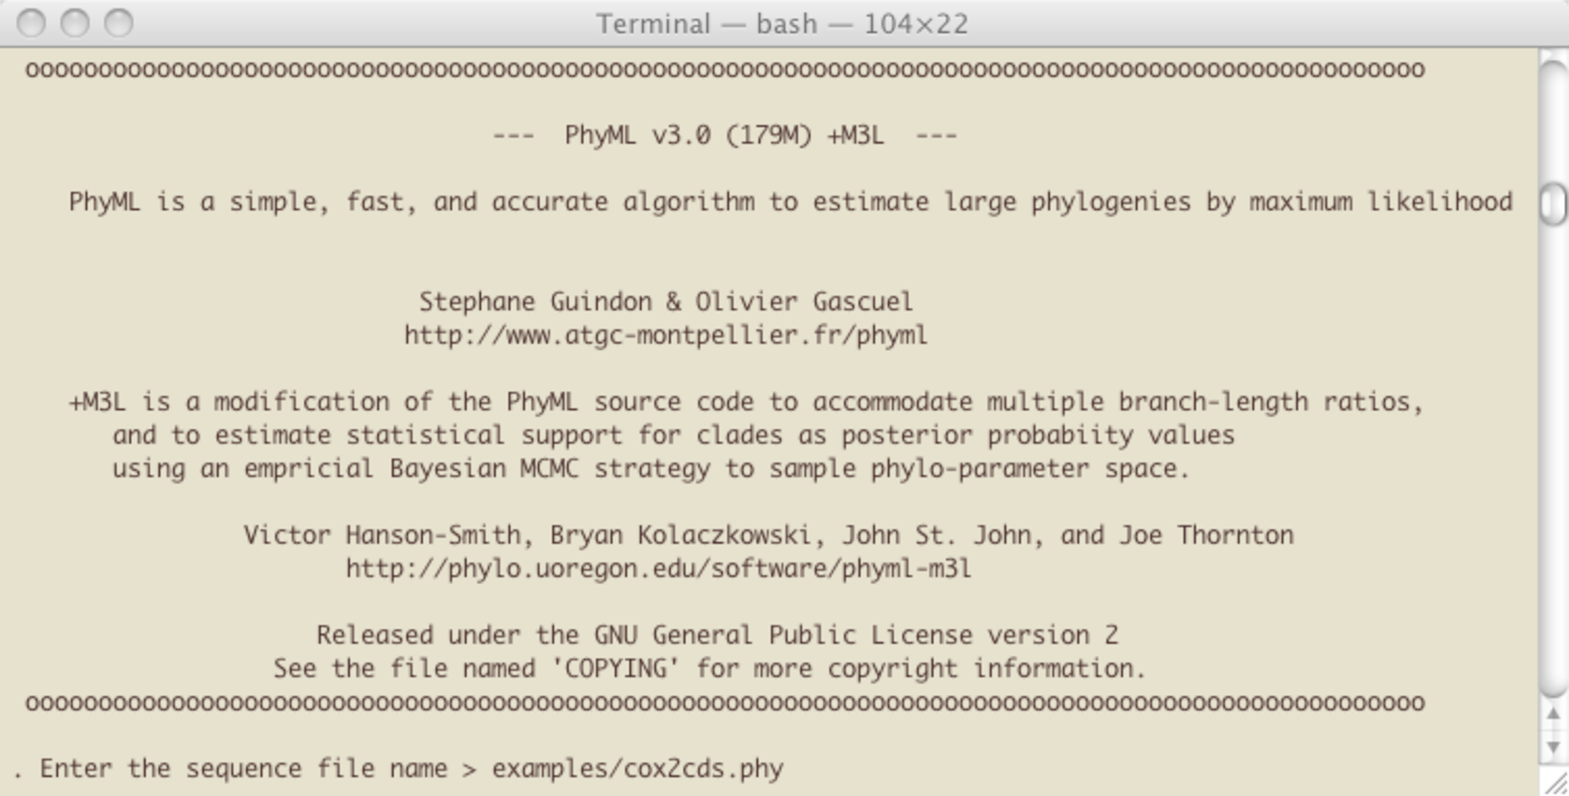
\includegraphics[width=5.5 in]{GRAPHICS/a1.pdf}
\caption{After PhyML+M3L loads, enter the filepath of the \textit{cox2cds.phy} alignment.}
\end{figure}
\clearpage

\begin{figure}[p]
\centering
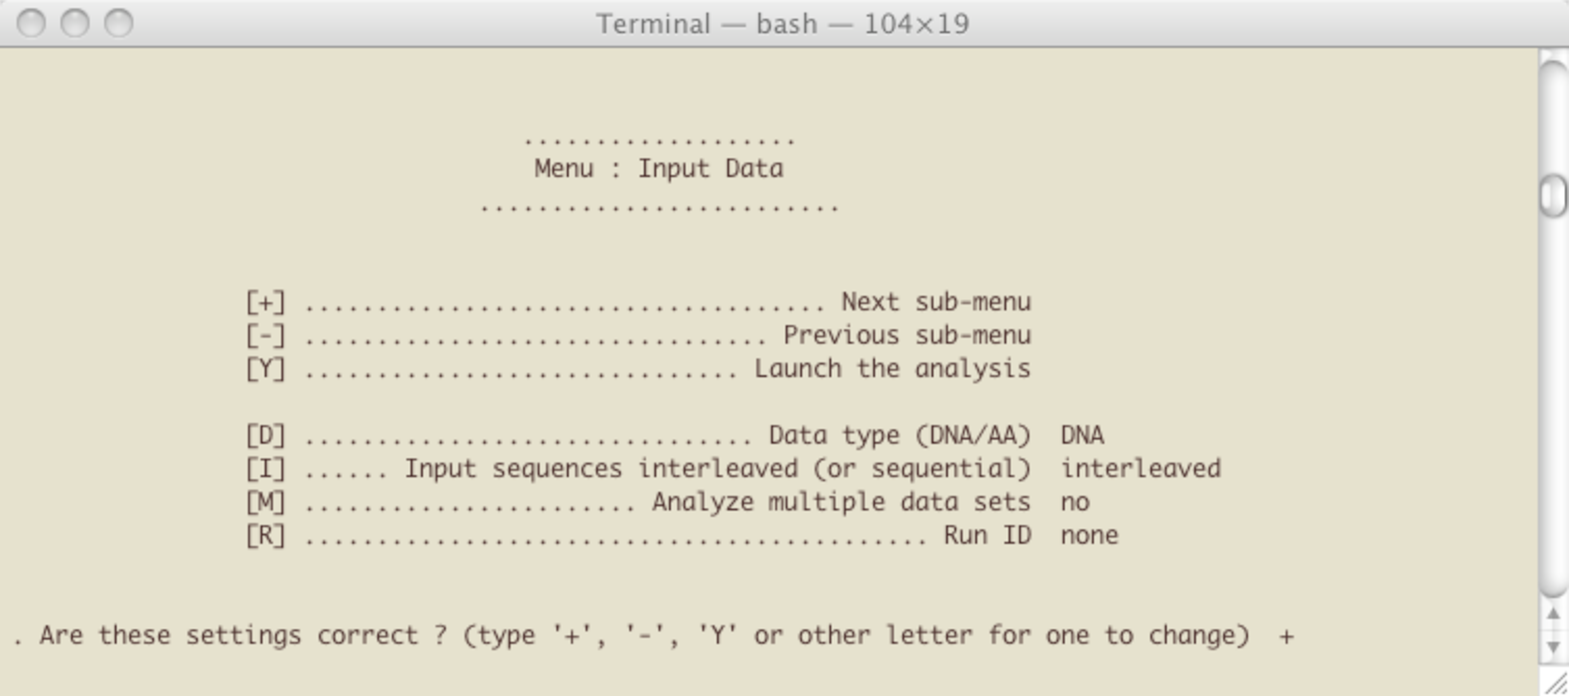
\includegraphics[width=5.5 in]{GRAPHICS/a2.pdf}
\caption{The Cox-2 data is DNA (nucleotide) data, so no changes need to be made on this menu page.  Enter `+' to advance to the next menu page.}
\end{figure}
\clearpage

\begin{figure}[p]
\centering
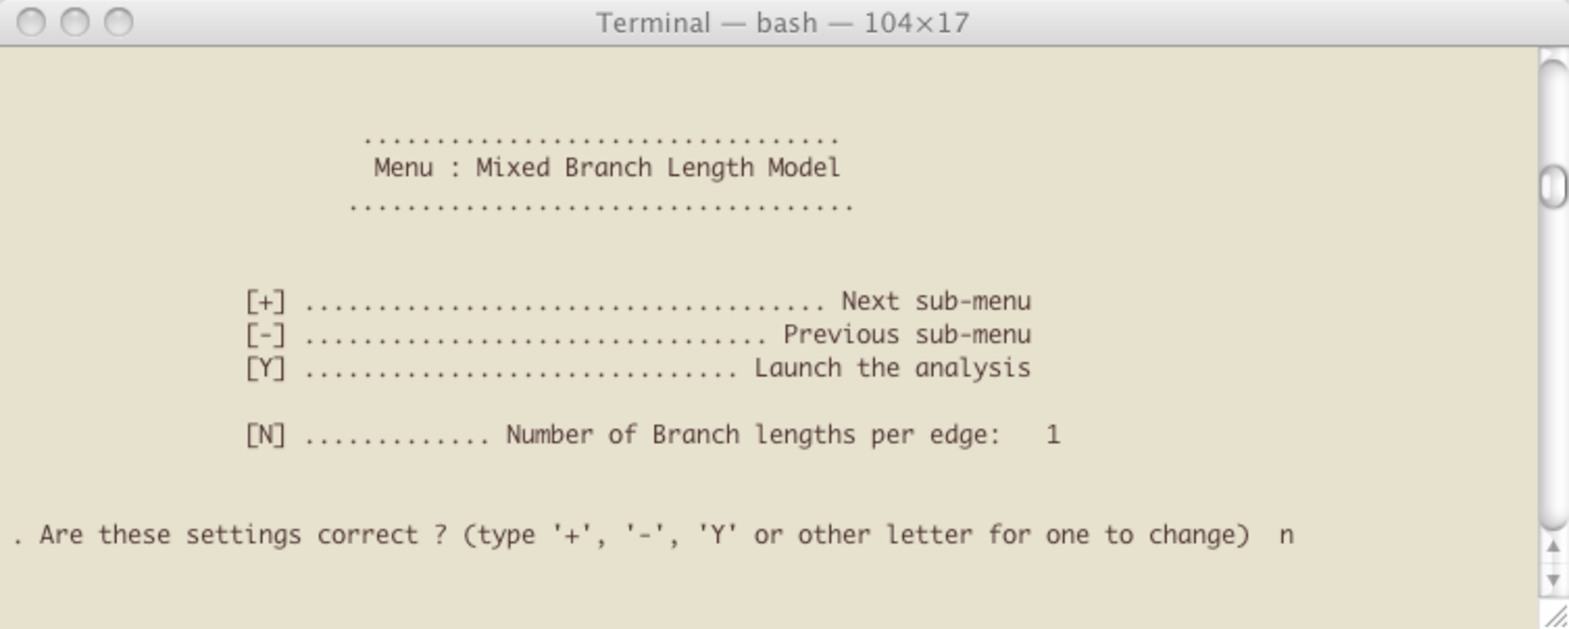
\includegraphics[width=5.5 in]{GRAPHICS/a3.pdf}
\caption{The mixed branch length model is disabled by default.  Enter `n' to enable the model and specify multiple branch lengths per edge.}
\end{figure}
\clearpage

\begin{figure}[p]
\centering
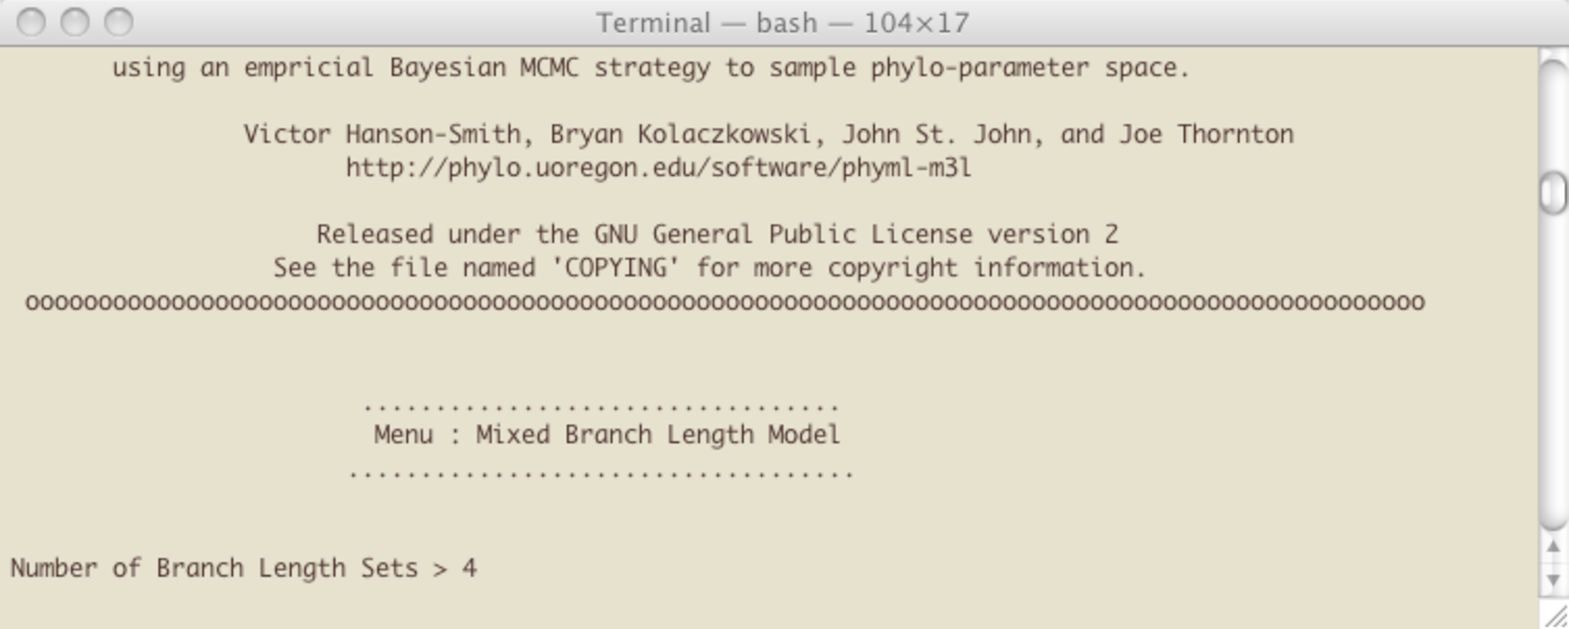
\includegraphics[width=5.5 in]{GRAPHICS/a4.pdf}
\caption{Enter `4' for the number of branch length sets.}
\end{figure}
\clearpage

\begin{figure}[p]
\centering
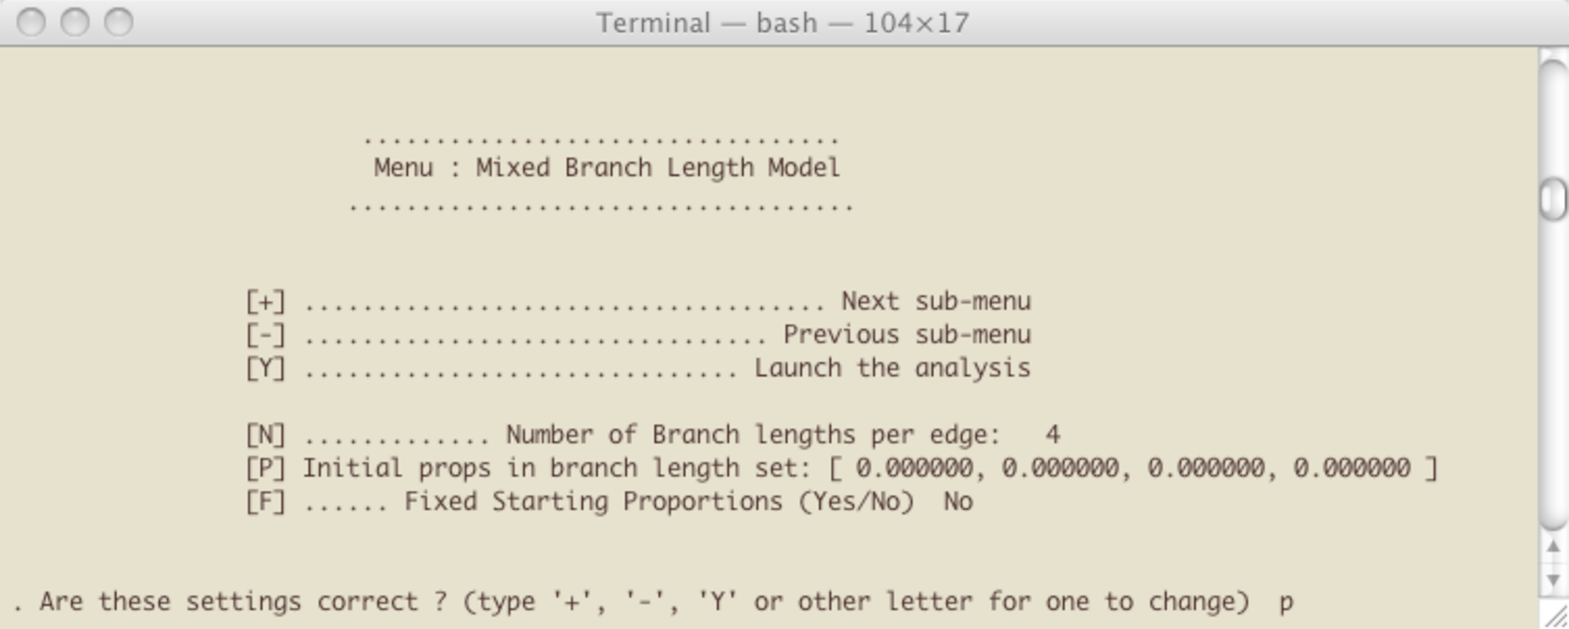
\includegraphics[width=5.5 in]{GRAPHICS/a5.pdf}
\caption{After you specify the number of branch length sets, you will automatically return to the menu.  Notice that some additional options now appear.  Next we'll specify the proportion of sites in each branch length category.  Enter `p'.}
\end{figure}
\clearpage

\begin{figure}[p]
\centering
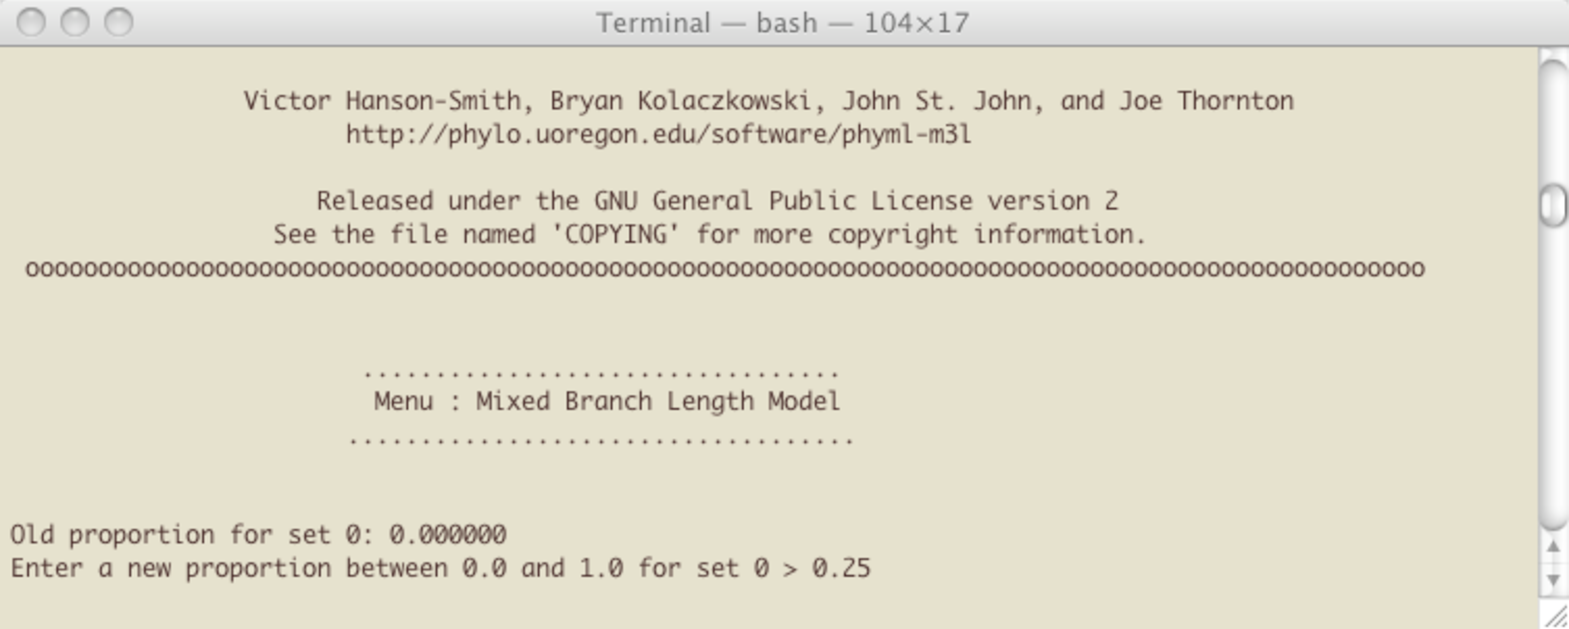
\includegraphics[width=5.5 in]{GRAPHICS/a6.pdf}
\caption{Enter `0.25' for each branch length proportion. }
\end{figure}
\clearpage

\begin{figure}[p]
\centering
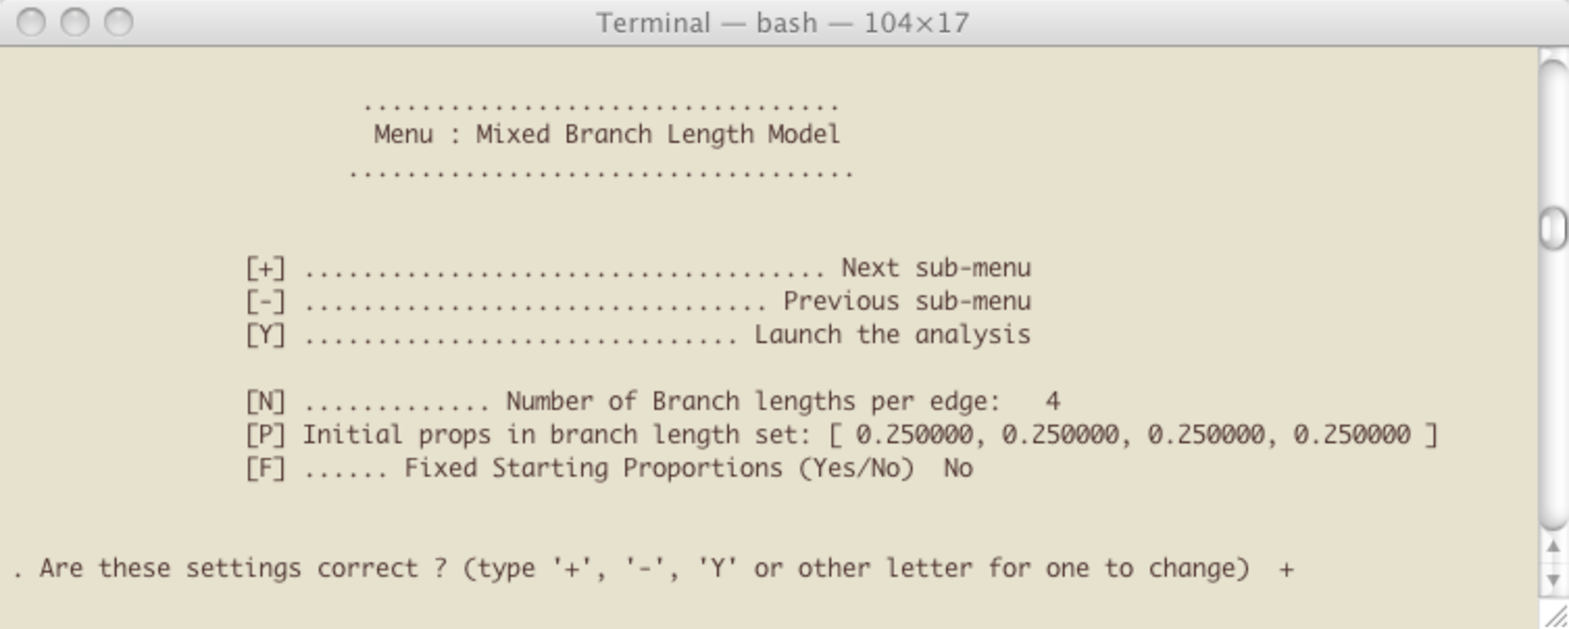
\includegraphics[width=5.5 in]{GRAPHICS/a7.pdf}
\caption{After specifying branch length proportions, you will automatically return to the menu.  Notice that your proportion specifications are now shown in the menu.  Enter `+' to advance to the next menu.}
\end{figure}
\clearpage

\begin{figure}[ph]
\centering
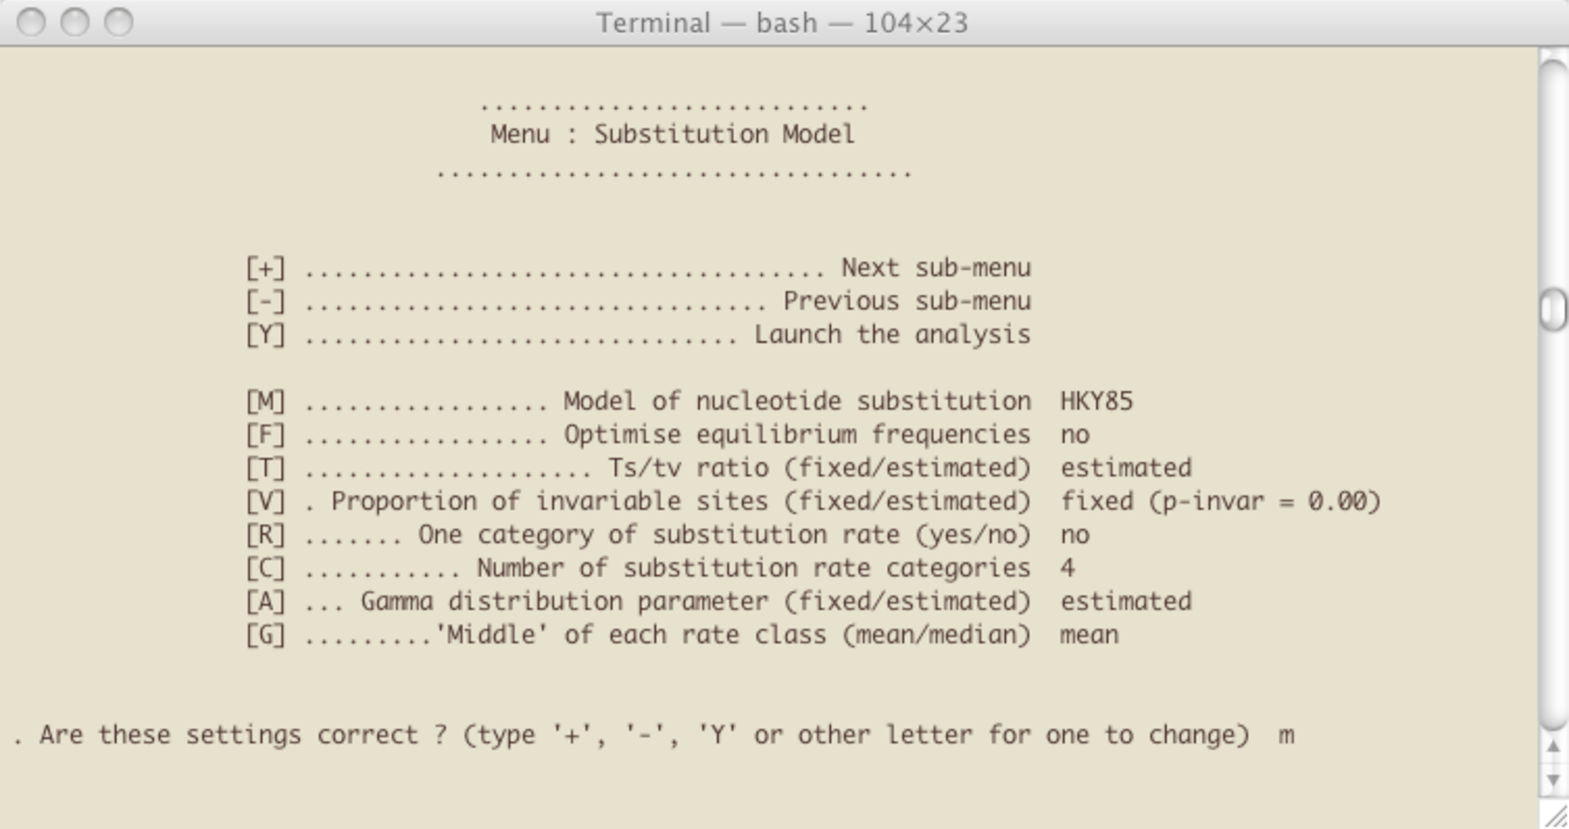
\includegraphics[width=5.5 in]{GRAPHICS/a8.pdf}
\caption{This menu allows you specify the substitution model.  By default, PhyML uses the HKY85 model for nucleotide data.  Instead, let's use the simpler JC69 model.  Enter `m' to cycle through the available model options.  Stop cycling when you see the model named `JC69'.}
\end{figure}
\clearpage

\begin{figure}[p]
\centering
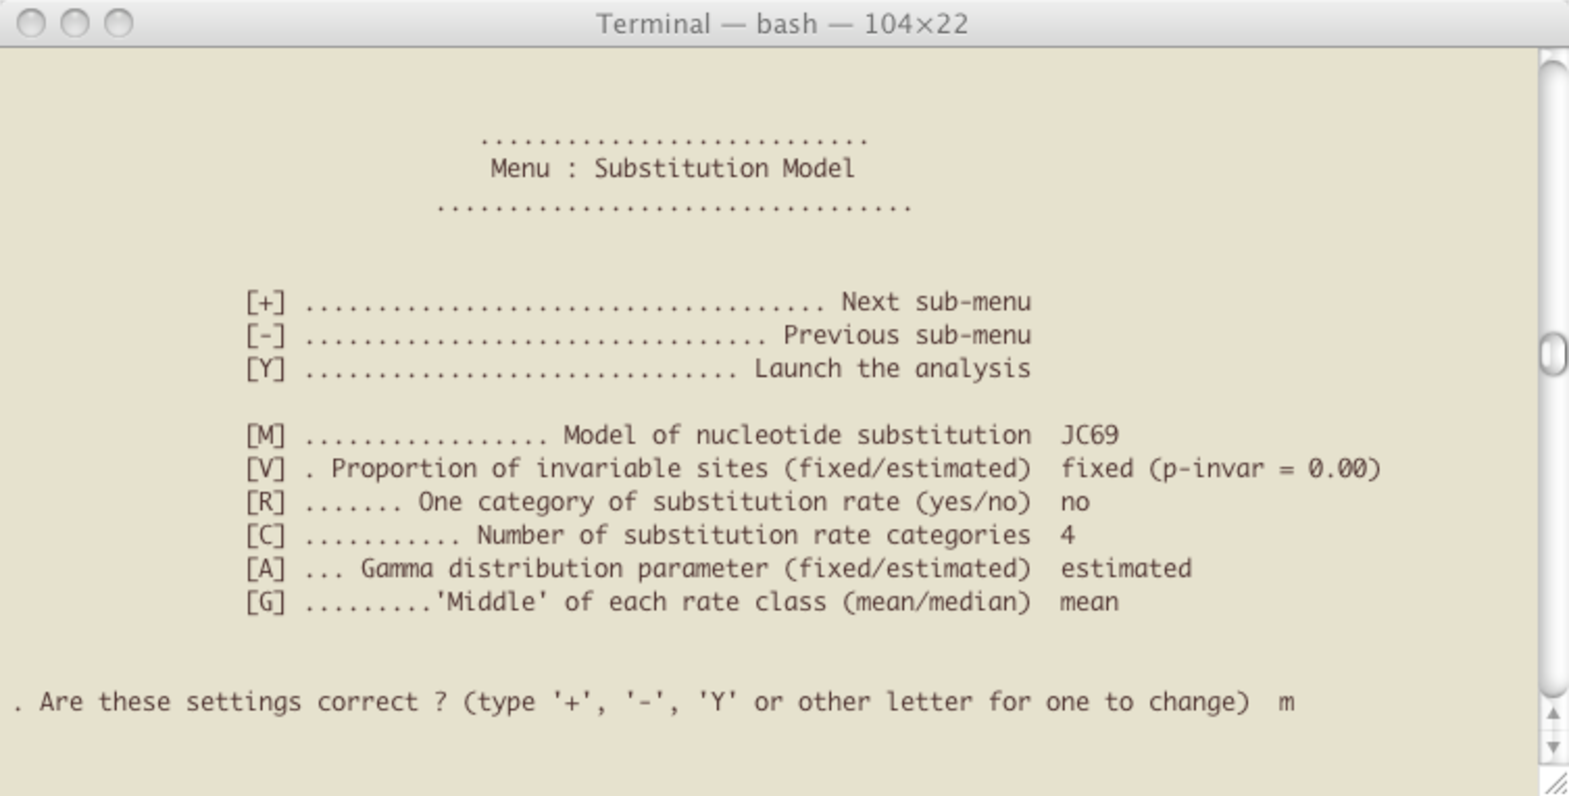
\includegraphics[width=5.5 in]{GRAPHICS/a9.pdf}
\caption{By default, PhyML uses four gamma-distributed evolutionary rates.  For this example, let's use a simpler model with only one evolutionary rate.  Enter `r' to disable the gamma-distributed model.}
\end{figure}
\clearpage

\begin{figure}[p]
\centering
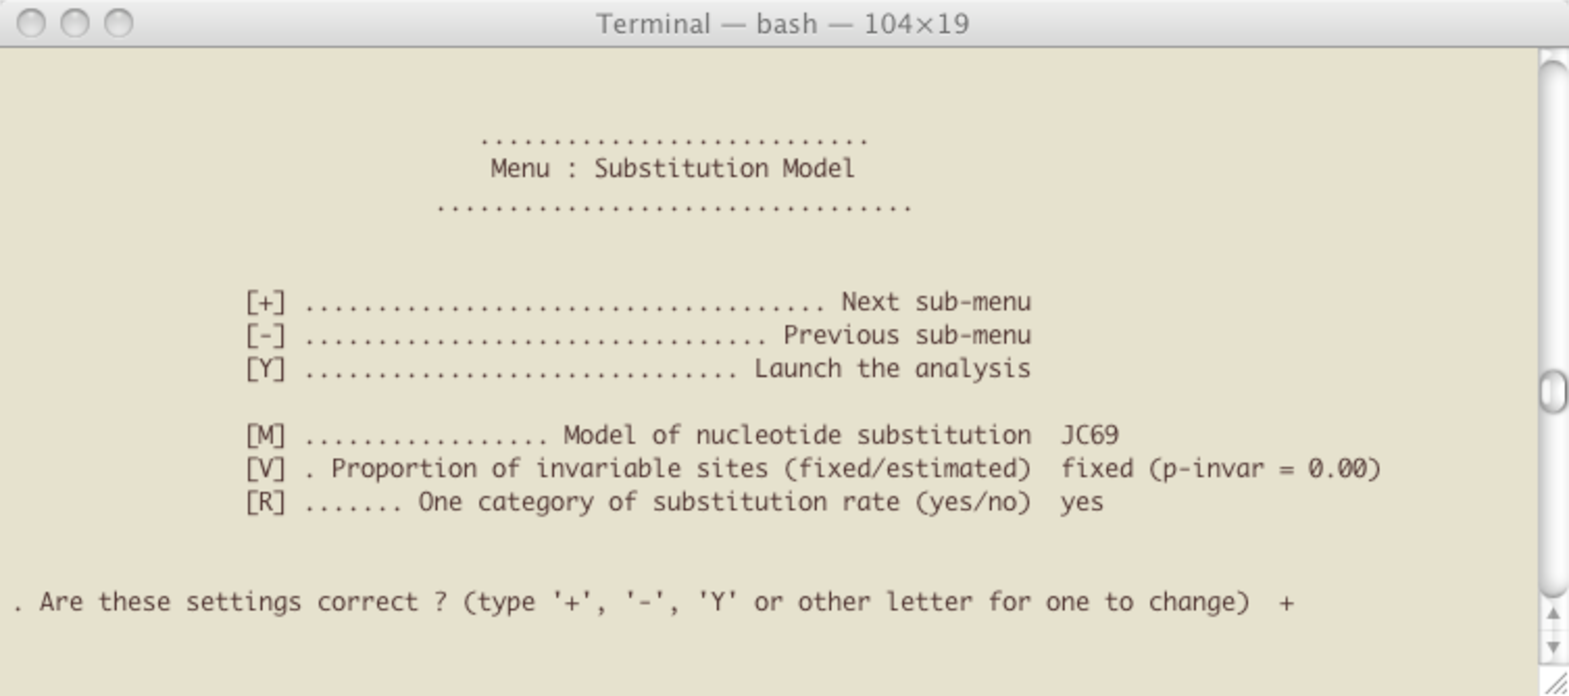
\includegraphics[width=5.5 in]{GRAPHICS/a10.pdf}
\caption{After disabling the gamma-distributed model, the menu should look like this.  Enter `+' to advance to the next menu.}
\end{figure}
\clearpage

\begin{figure}[p]
\centering
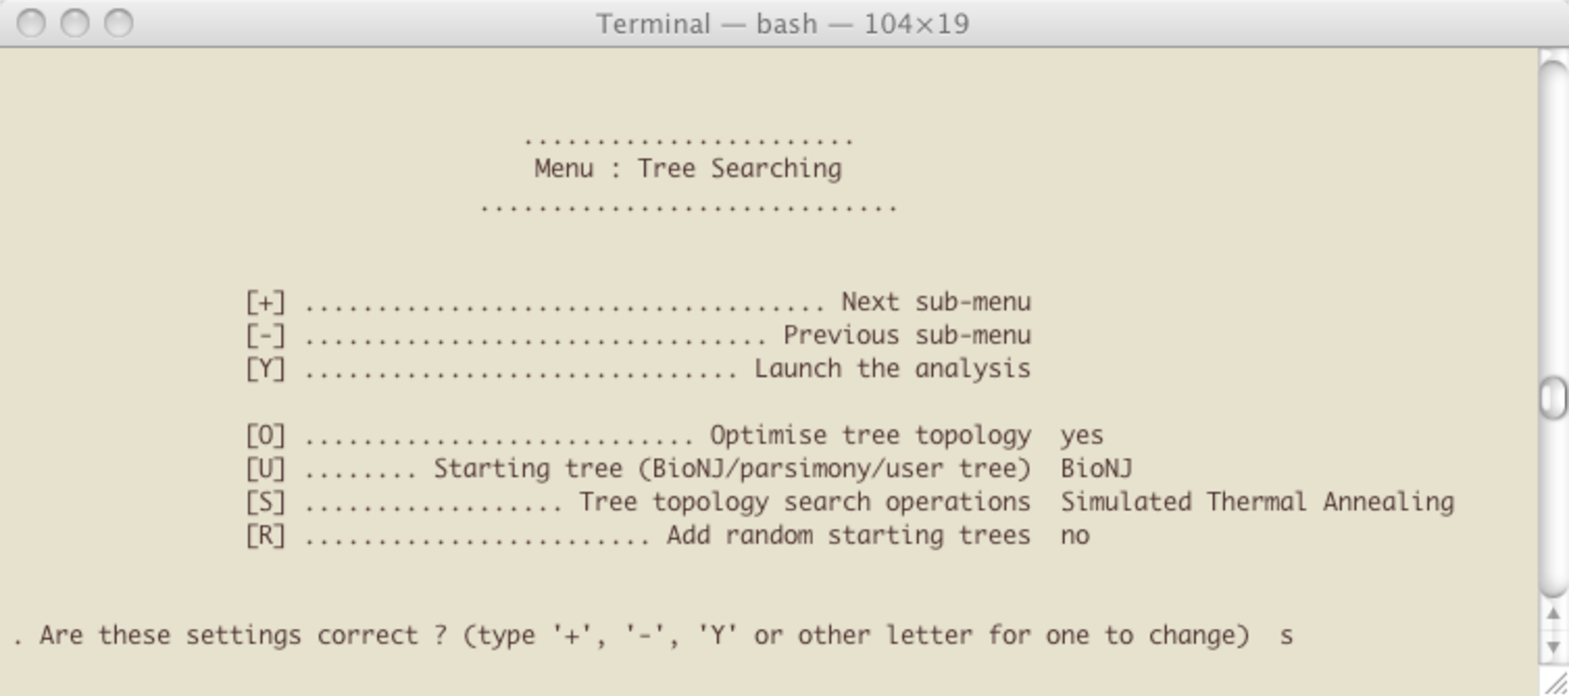
\includegraphics[width=5.5 in]{GRAPHICS/a11.pdf}
\caption{When using multiple branch lengths, PhyML+M3L enables simulated thermal annealing by default.  For this example, let's instead use hill-climbing with subtree pruning and regrafting.  Enter `s' to cycle through the search options.  Stop cycling when you see the option named `SPR moves (slow, accurate)'.}
\end{figure}
\clearpage

%\begin{figure}[p]
%\centering
%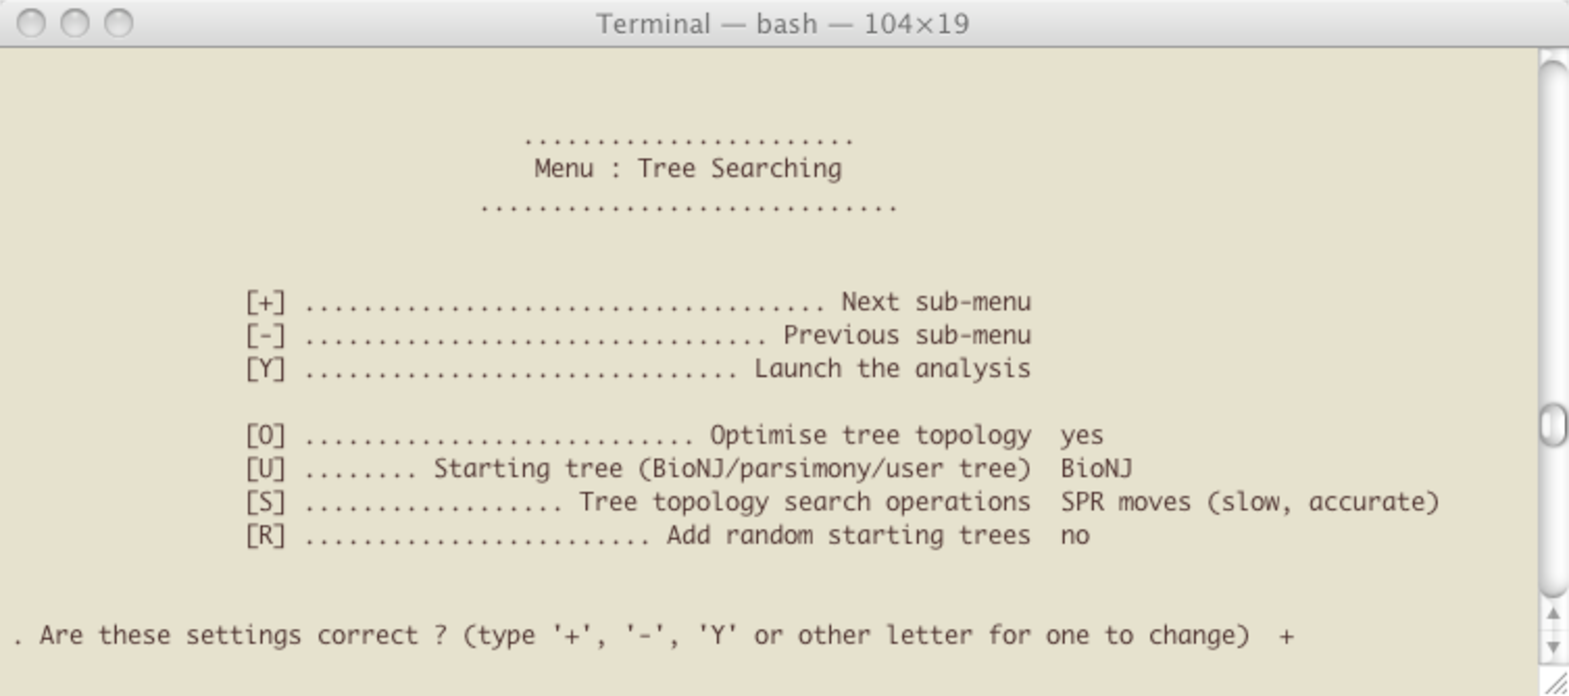
\includegraphics[width=5.5 in]{GRAPHICS/a12.pdf}
%
%\end{figure}
%\clearpage

\begin{figure}[p]
\centering
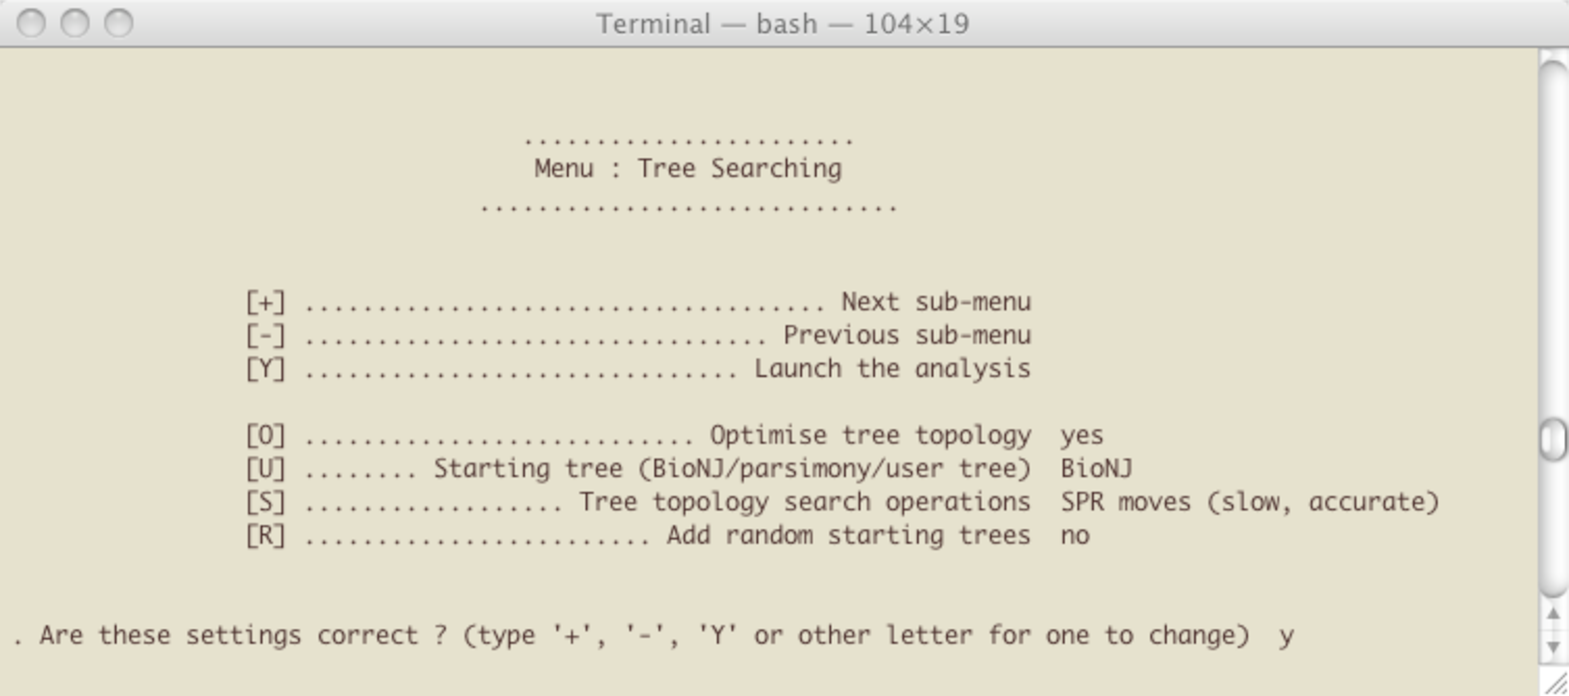
\includegraphics[width=5.5 in]{GRAPHICS/a13.pdf}

\caption{After selecting SPR, the menu should like this.  Although there exist other menu options we could consider, let's start the analysis.  Enter `y' to begin.}
\end{figure}
\clearpage

\begin{figure}[p]
\centering
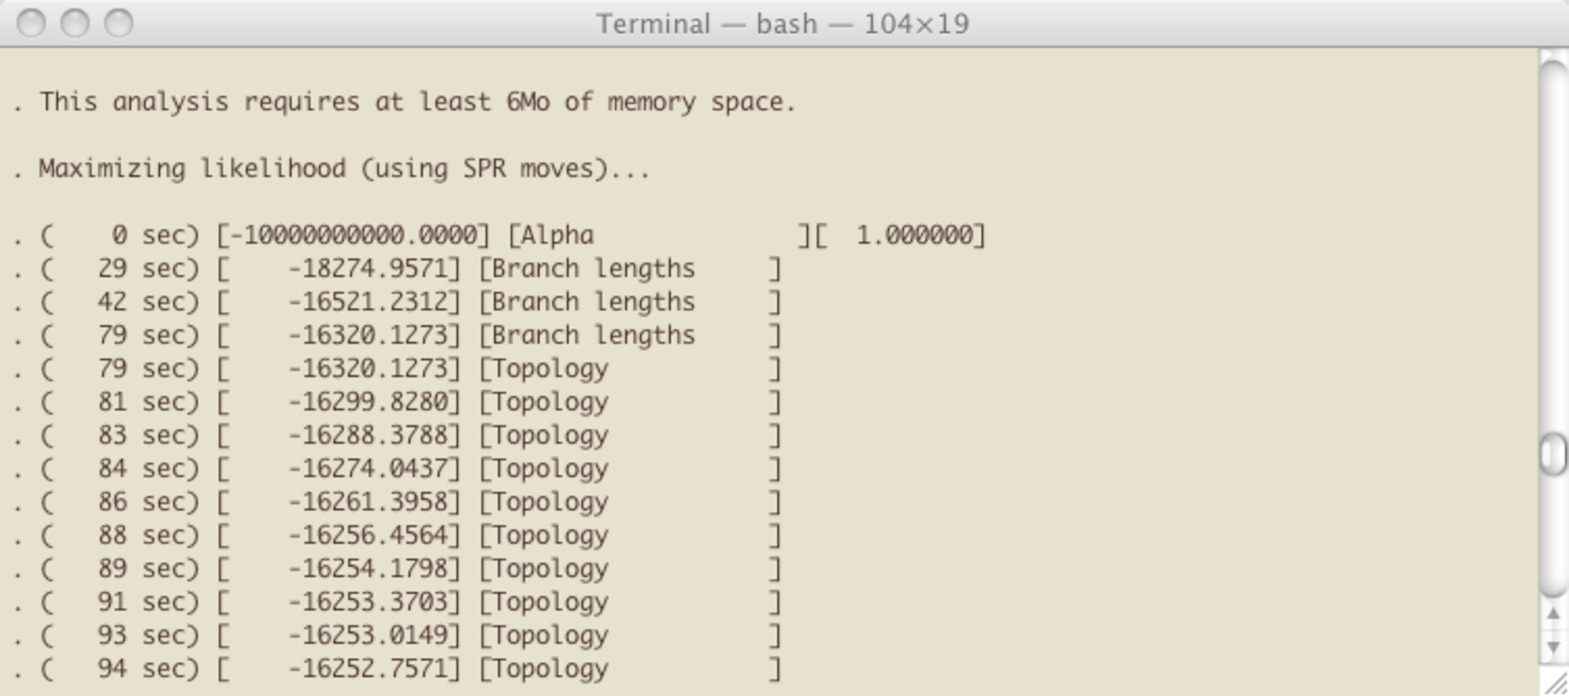
\includegraphics[width=5.5 in]{GRAPHICS/a14.pdf}
\caption{After entering `y', you should see output looking similar to this.  The actual numbers will likely be different.  Each row of this output displays (1) the total time used, (2) the log likelihood of the current phylogeny, and (3) the parameter that was modified to find this tree.  This output will be grow until the hill-climbing algorithm converges on a likelihood maxima.  Be patient, the analysis can take a while.}
\end{figure}
\clearpage

\begin{figure}[p]
\centering
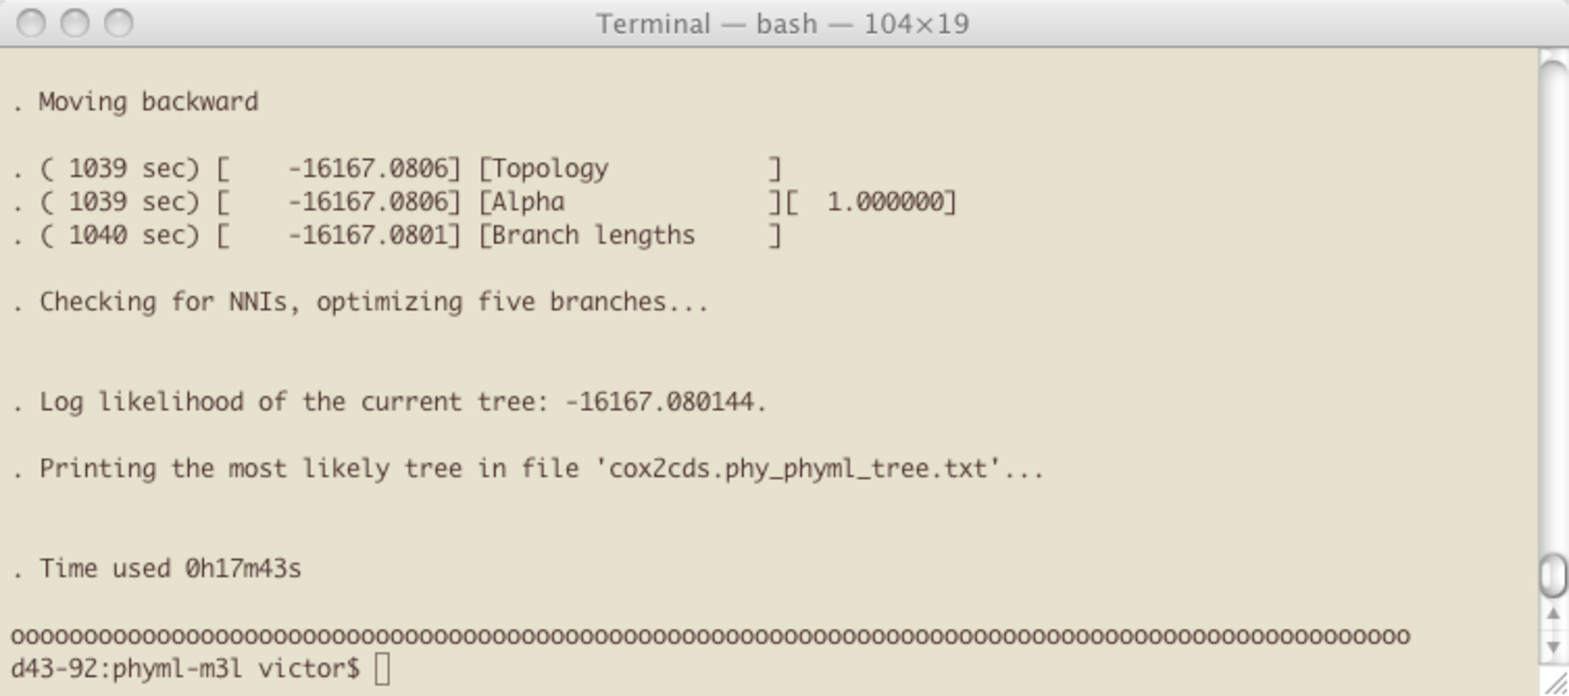
\includegraphics[width=5.5 in]{GRAPHICS/a15.pdf}
\caption{Eventually the analysis will finish, and you should see output that looks similar to this.  In this example, the best-found phylogeny has a log-likelihood of -16167.080144.  On a dual-core Intel MacBook, the analysis required 17 minutes and 43 seconds.  On your computer, perhaps it will take less time.}
\end{figure}
\clearpage

\begin{figure}[p]
\centering
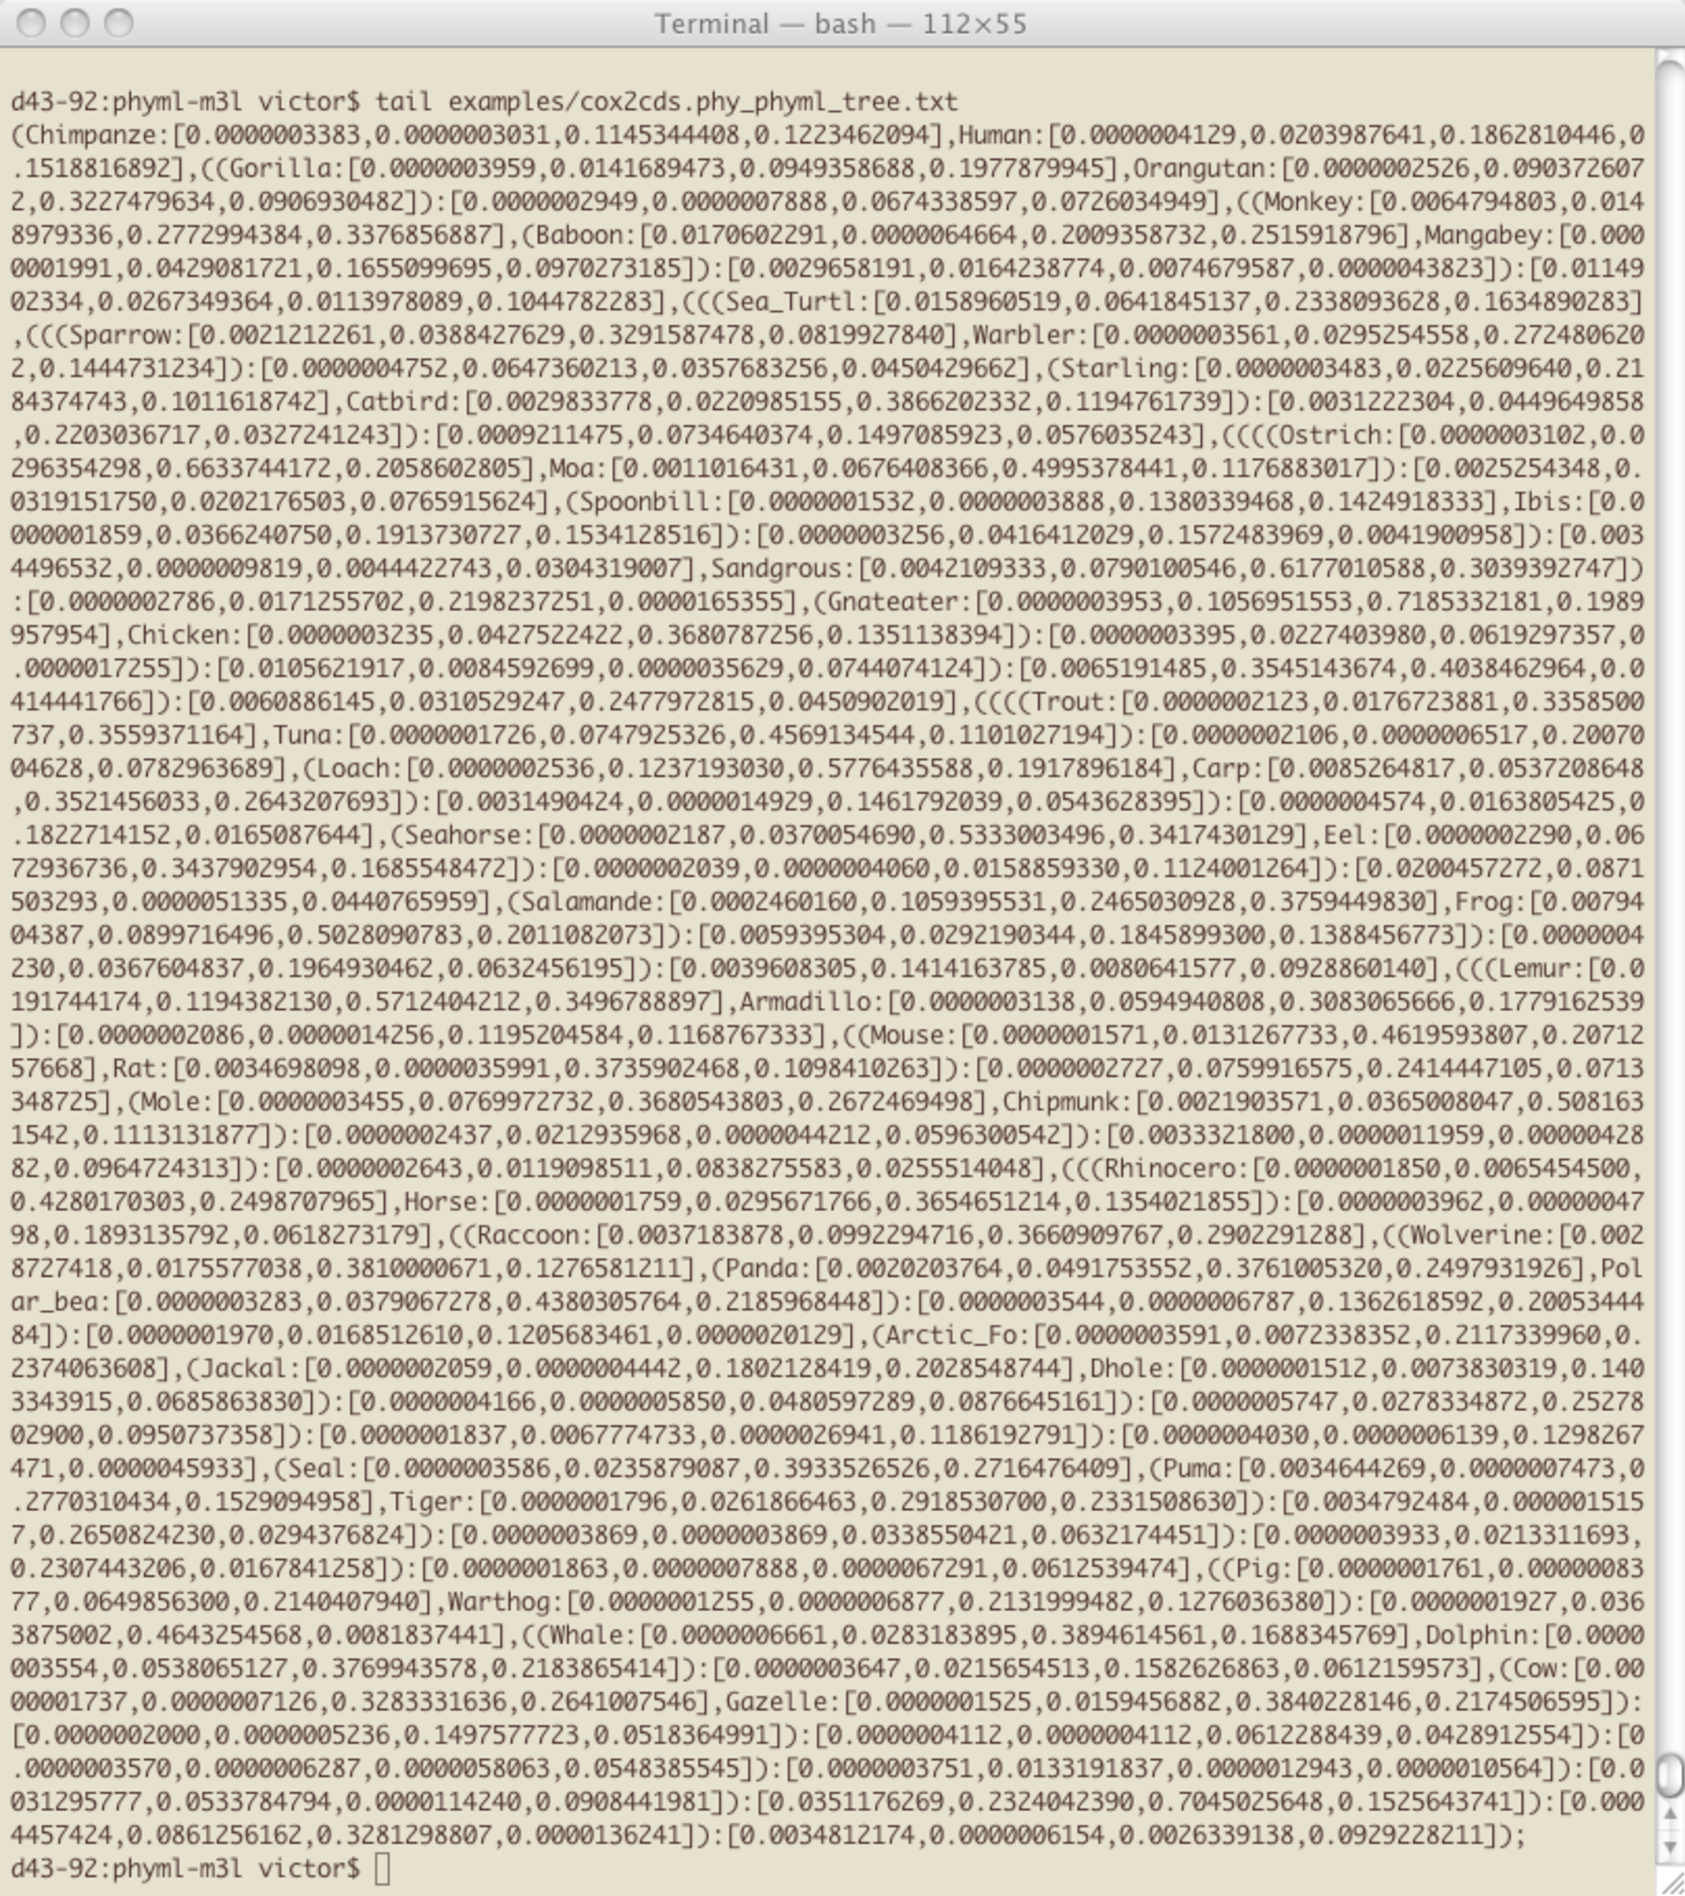
\includegraphics[width=5.5 in]{GRAPHICS/a16.pdf}
\caption{The resulting phylogeny is printed as a Newick-formatted string in a text file.  You can view that text file using your favorite text editor, or using unix commands such as \textit{tail}, \textit{less}, or \textit{cat}.  Notice that each branch has four length values wrapped in brackets `[' and `]'.}
\end{figure}
\clearpage

\pagebreak
\subsection{Using empirical Bayes MCMC to estimate clade support}

Begin by navigating to the folder that contains the PhyML+M3L program.  This folder should contain a subfolder named \textit{examples}, in which the \textit{cox2cds.phy} alignment is located.

\begin{figure}[h]
\centering
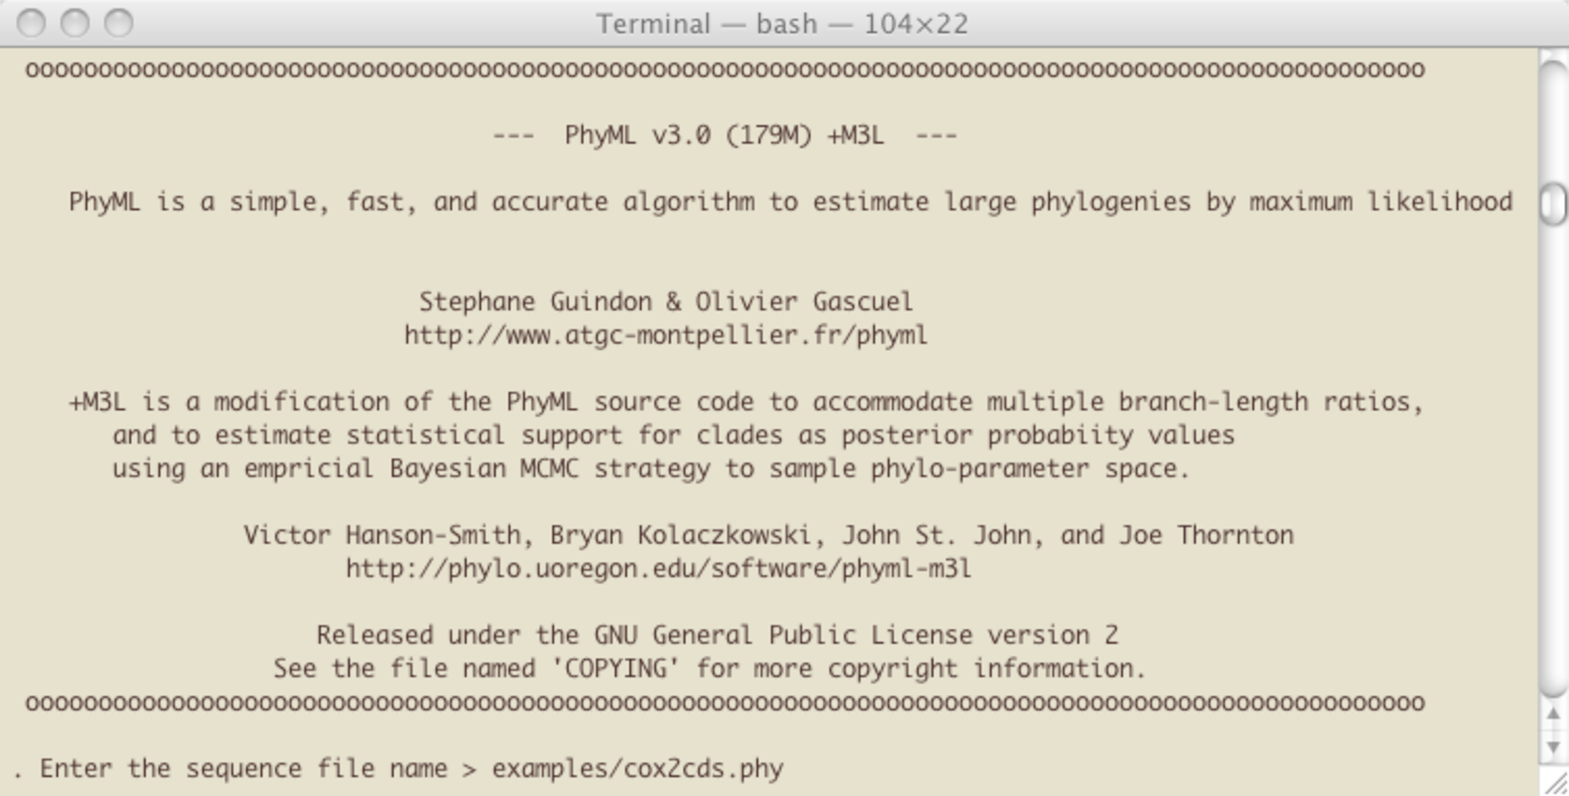
\includegraphics[width=5.5 in]{GRAPHICS/a1.pdf}
\caption{After PhyML+M3L loads, enter the filepath of the \textit{cox2cds.phy} alignment.}
\end{figure}
\clearpage

\begin{figure}[p]
\centering
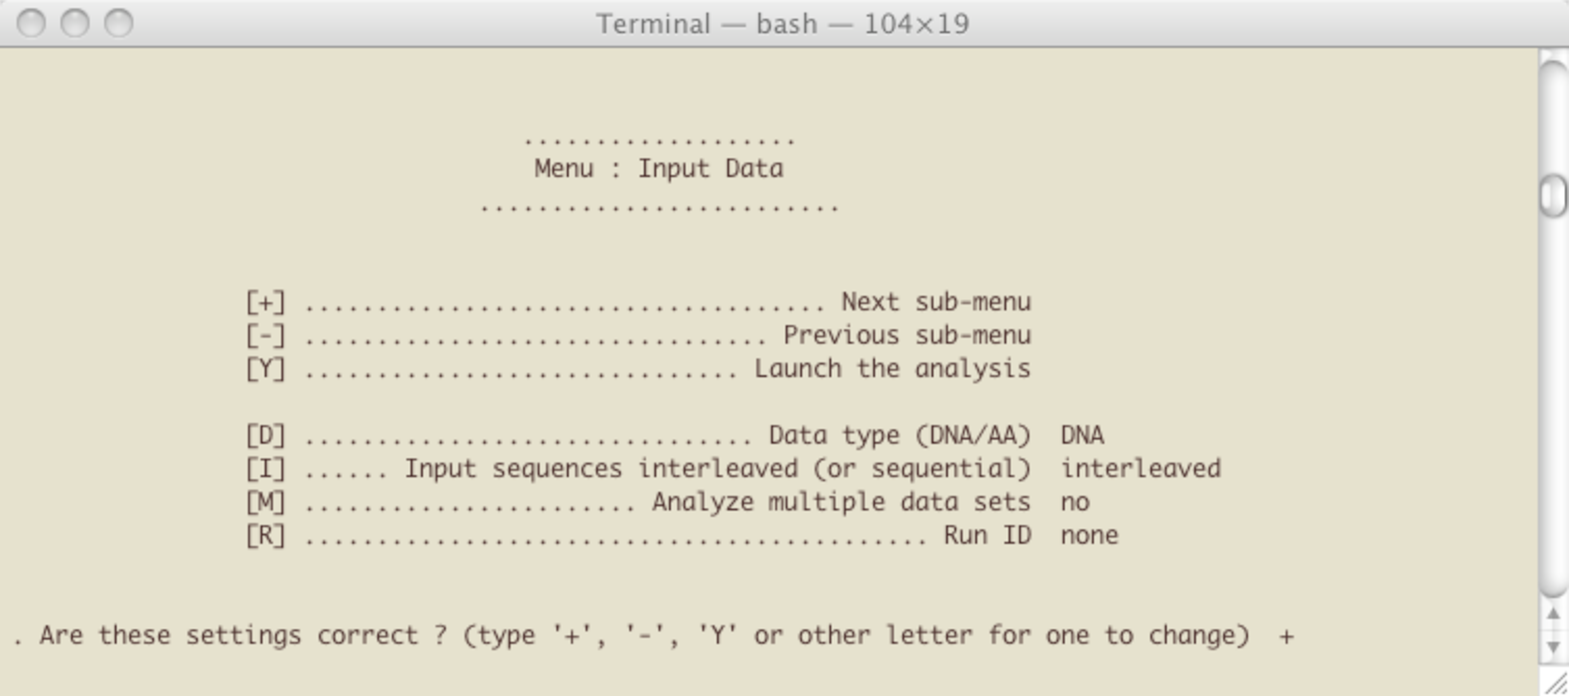
\includegraphics[width=5.5 in]{GRAPHICS/a2.pdf}
\caption{The Cox-2 data is DNA (nucleotide) data, so no changes need to be made on this menu page.  Enter `+' to advance to the next menu page.}
\end{figure}
\clearpage

\begin{figure}[p]
\centering
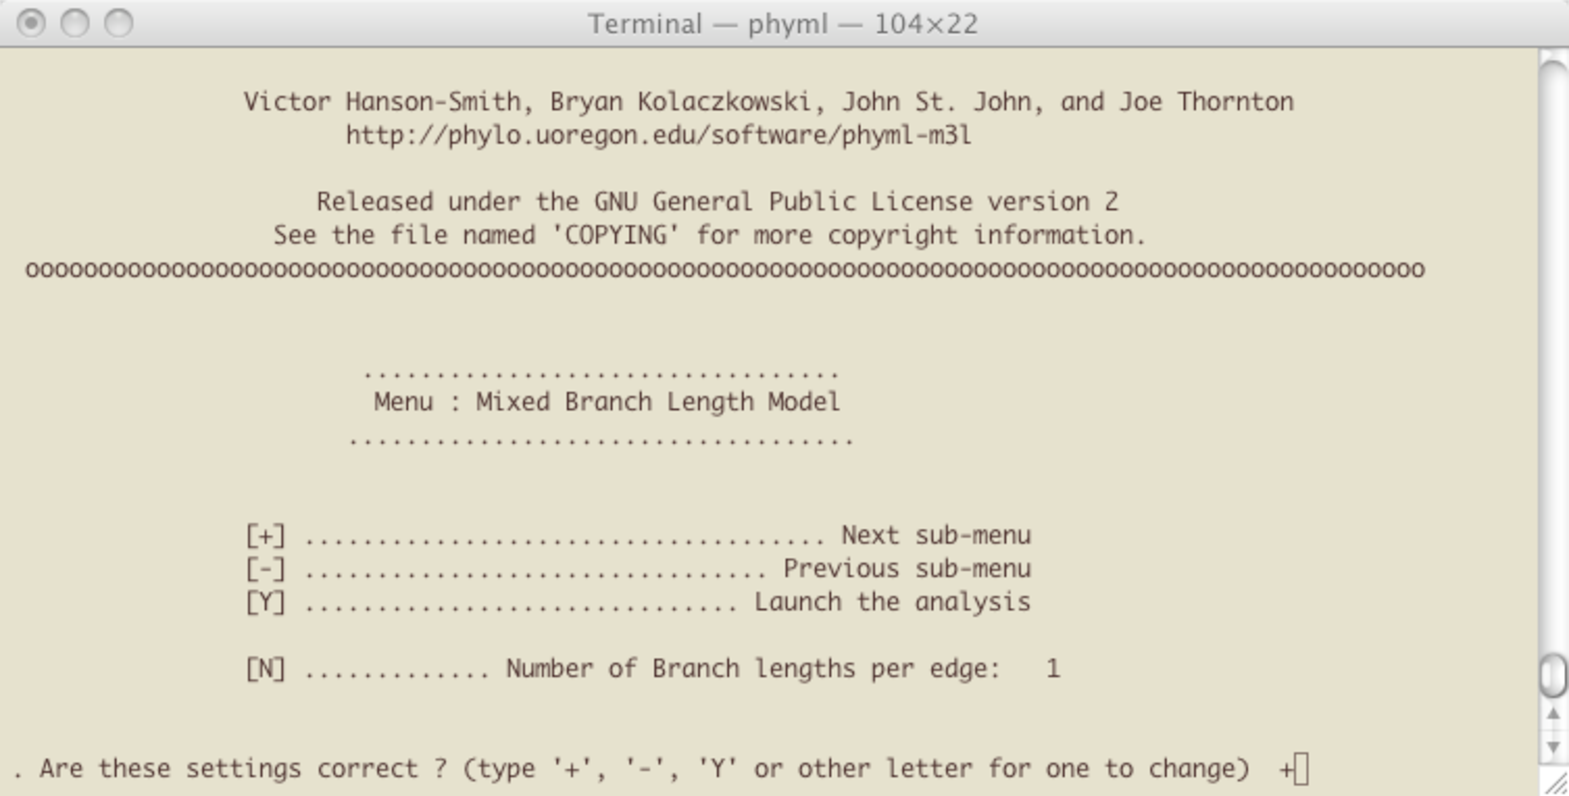
\includegraphics[width=5.5 in]{GRAPHICS/b1.pdf}
\caption{For this example, we'll use only one branch length set.  Leave this menu alone and enter `+' to advance to the next menu.}
\end{figure}
\clearpage

\begin{figure}[ph]
\centering
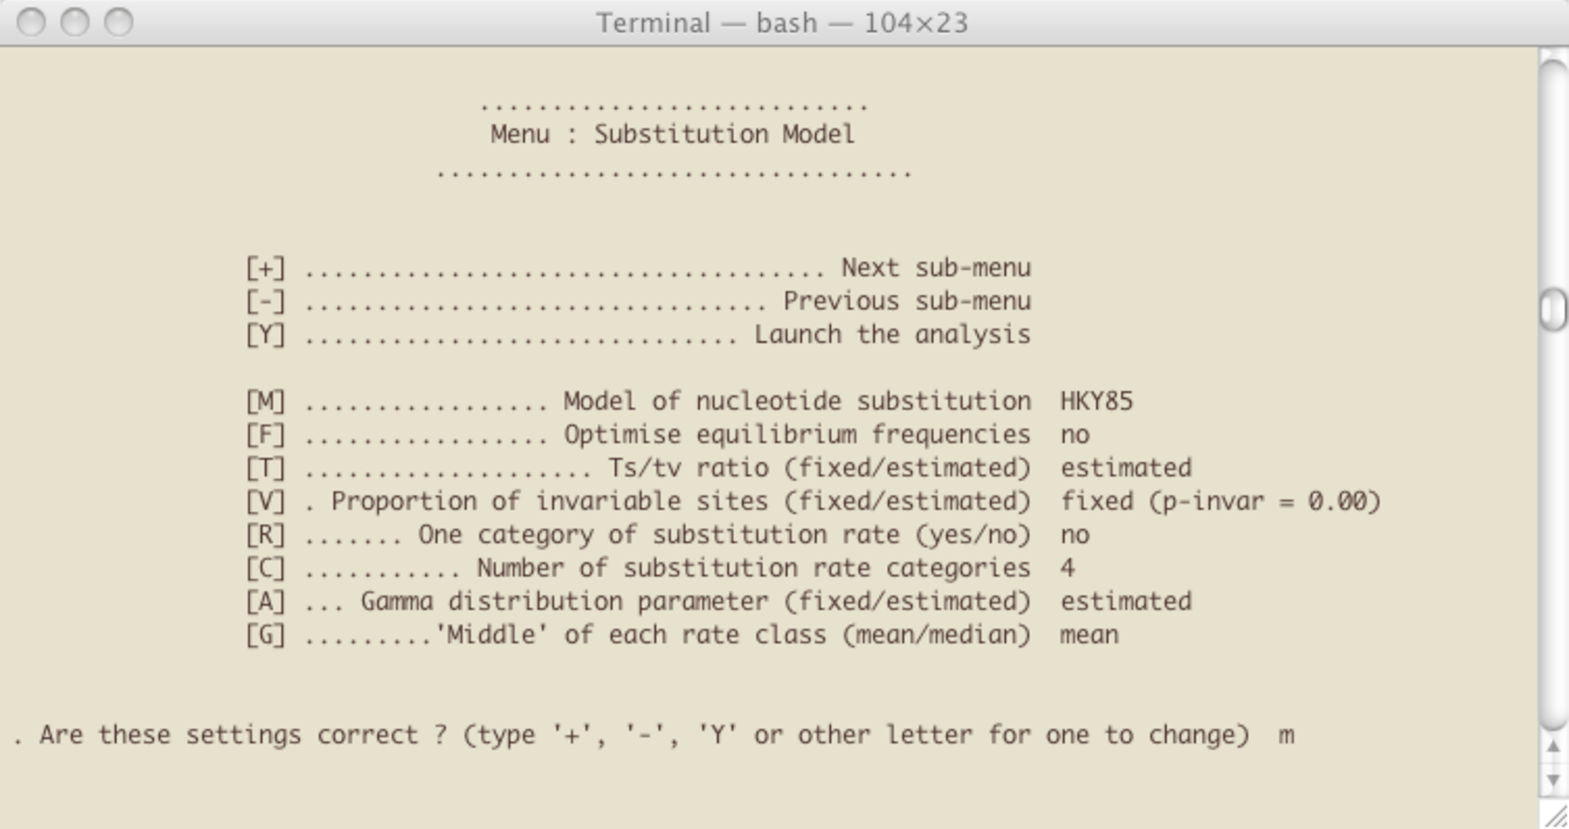
\includegraphics[width=5.5 in]{GRAPHICS/a8.pdf}
\caption{This menu allows you specify the substitution model.  By default, PhyML uses the HKY85 model for nucleotide data.  Instead, let's use the simpler JC69 model.  Enter `m' to cycle through the available model options.  Stop cycling when you see the model named `JC69'.  Also, enter `r' to disable the gamma-distributed rates model.}
\end{figure}
\clearpage

\begin{figure}[p]
\centering
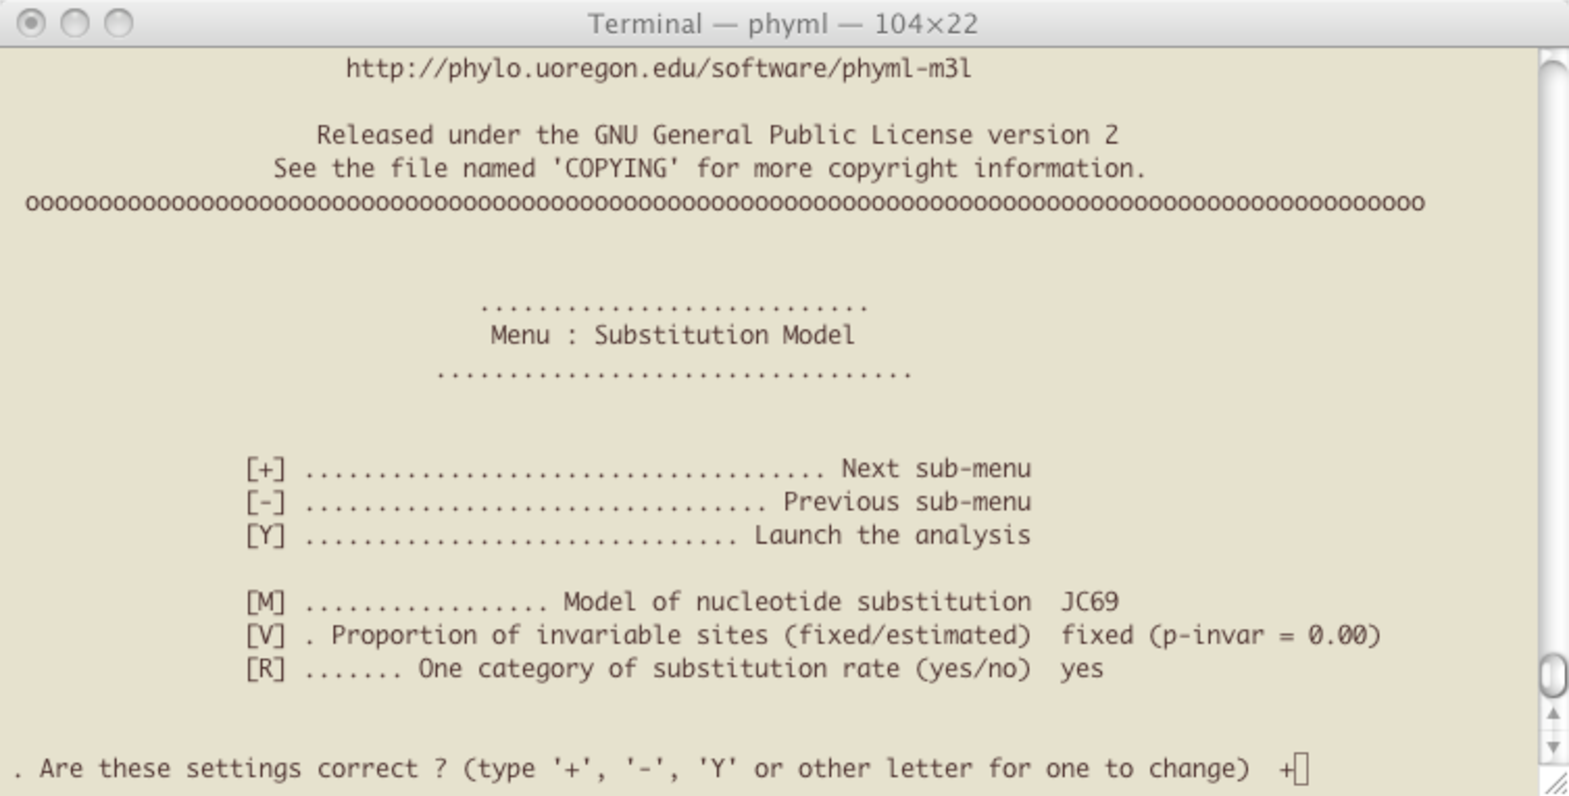
\includegraphics[width=5.5 in]{GRAPHICS/b2.pdf}
\caption{At this point, the menu should look like this.  Enter `+' to advance to the next menu.}
\end{figure}
\clearpage

\begin{figure}[p]
\centering
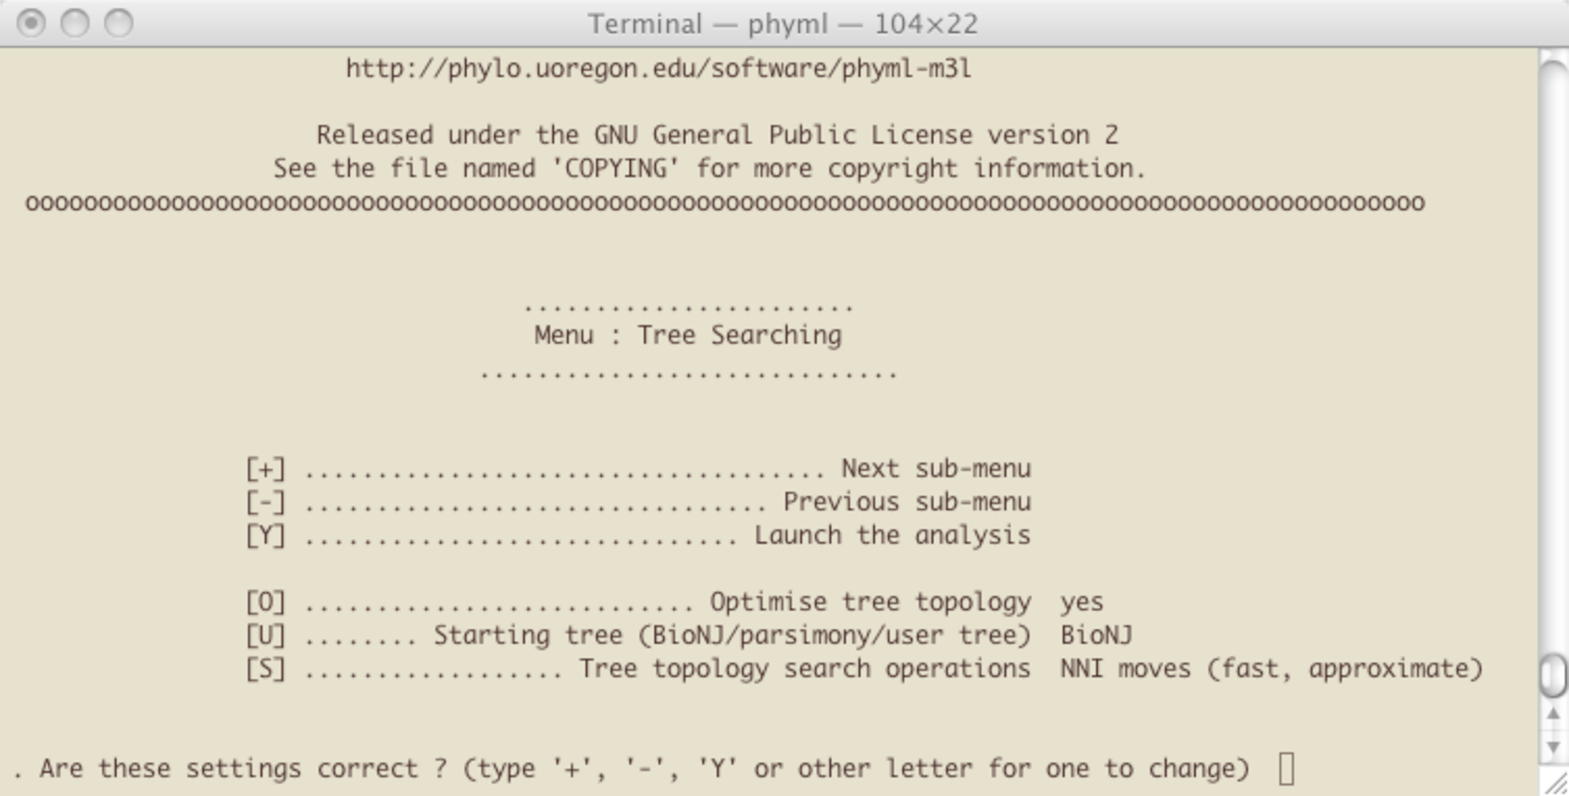
\includegraphics[width=5.5 in]{GRAPHICS/b3.pdf}
\caption{By default, PhyML uses a tree searching strategy based on nearest neighbor interchange (NNI) or subtree pruning and regrafting (SPR).  To enable empirical Bayes MCMC, enter `s' to cycle through the options.  Stop cycling when you see `Empirical Bayes MCMC'}
\end{figure}
\clearpage

\begin{figure}[p]
\centering
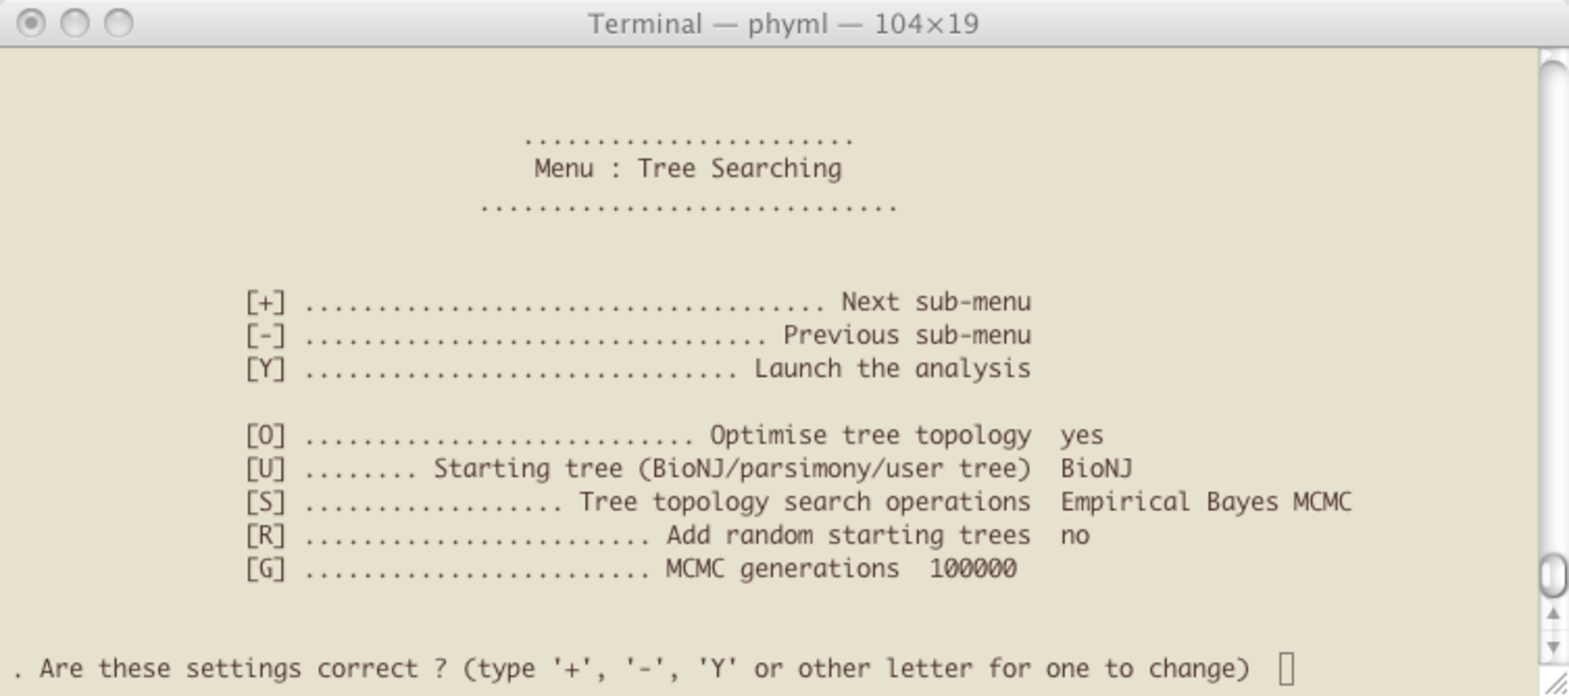
\includegraphics[width=5.5 in]{GRAPHICS/b4.pdf}
\caption{Notice that new options appear when you select empirical Bayes.  The option named `MCMC generations' specifies how many generations to run the MCMC analysis.  More generations will lead to a more accurate estimate of posterior probability values.  However, more generations will take more time.  By default, PhyML+M3L uses 100,000 generations.  For most practical analysis, we consider 100,000 to be a minimum number of generations to yield an accurate sample.  Enter `y' to start the analysis.}
\end{figure}
\clearpage

\begin{figure}[p]
\centering
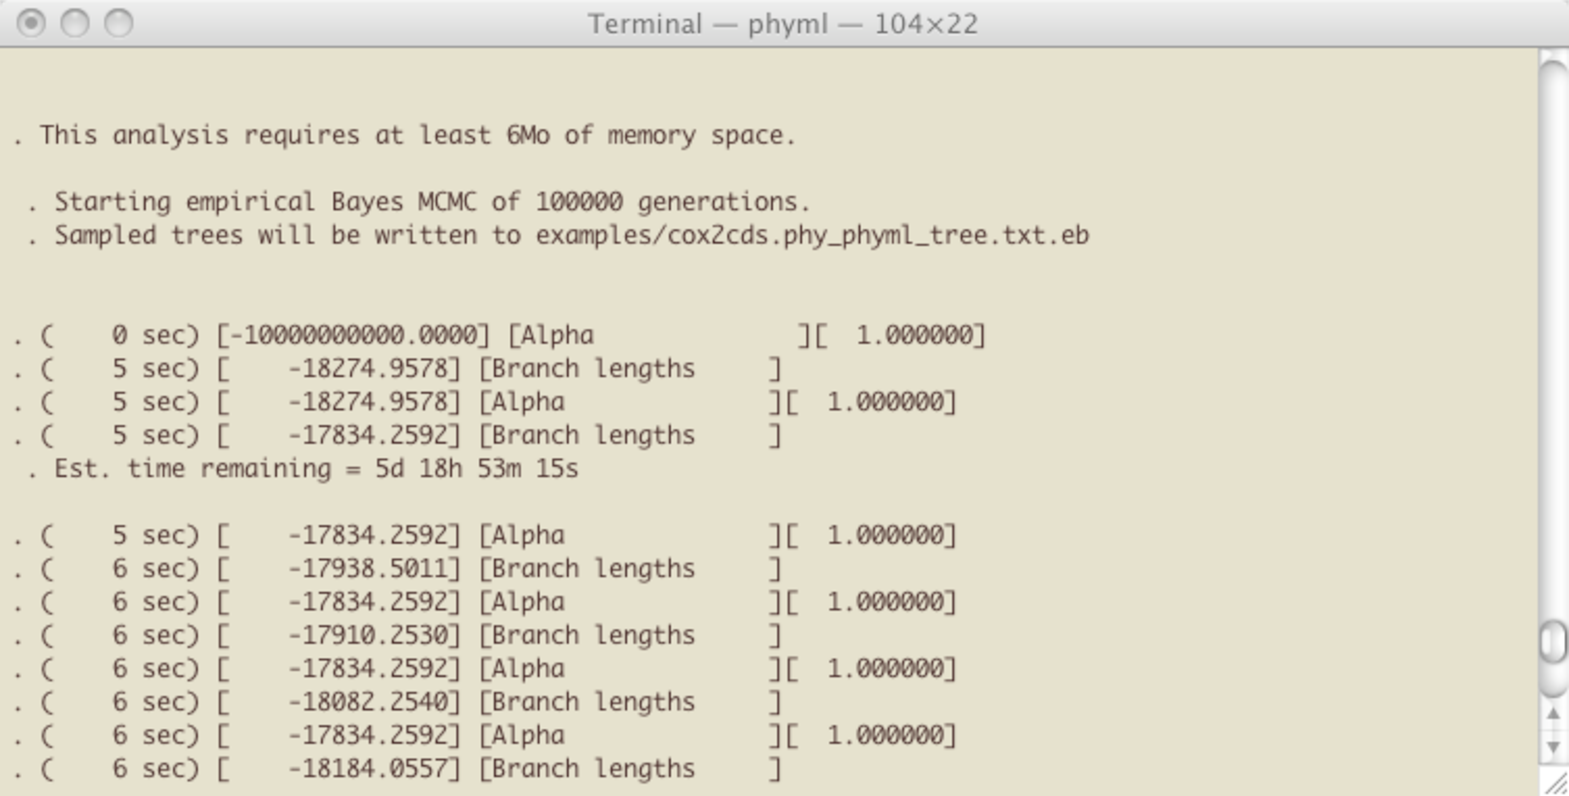
\includegraphics[width=5.5 in]{GRAPHICS/b5.pdf}
\caption{Once the analysis begins, you will see output that looks like this.  MCMC analysis can be very time consuming, so be patient.  If the estimated time remaining is large, we strongly suggest you run the analysis on a computer that remains powered-on with few computational distractions.  If  you are use PhyML+M3L on a remote cluster, we encourage you to learn about the unix command named \textit{screen} (it allows you to continue running the job after you logout).}
\end{figure}
\clearpage

\begin{figure}[p]
\centering
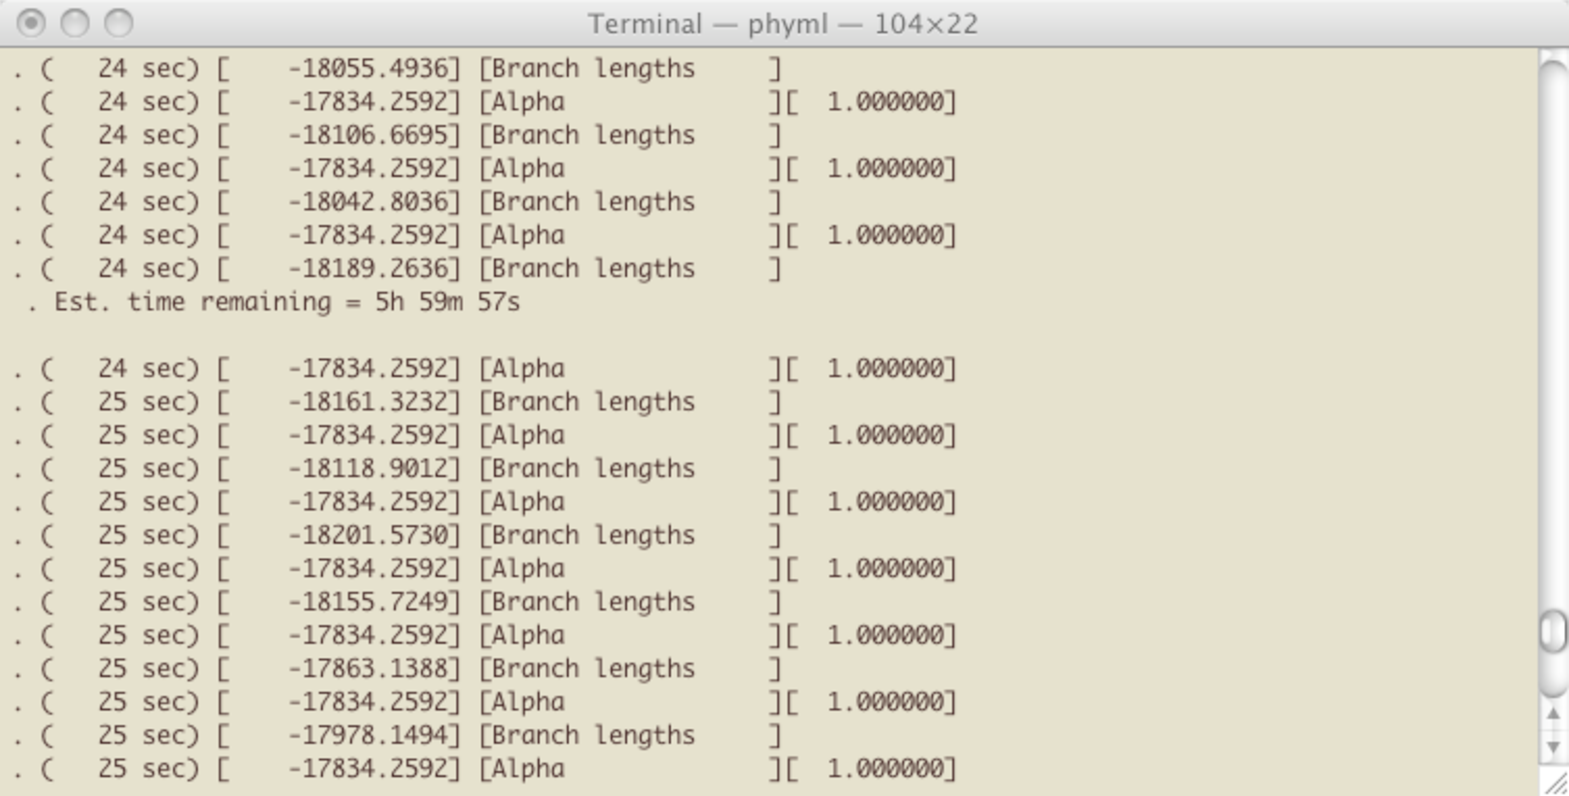
\includegraphics[width=5.5 in]{GRAPHICS/b6.pdf}
\caption{As the analysis continues, the estimate time remaining will decrease.}
\end{figure}
\clearpage

\begin{figure}[p]
\centering
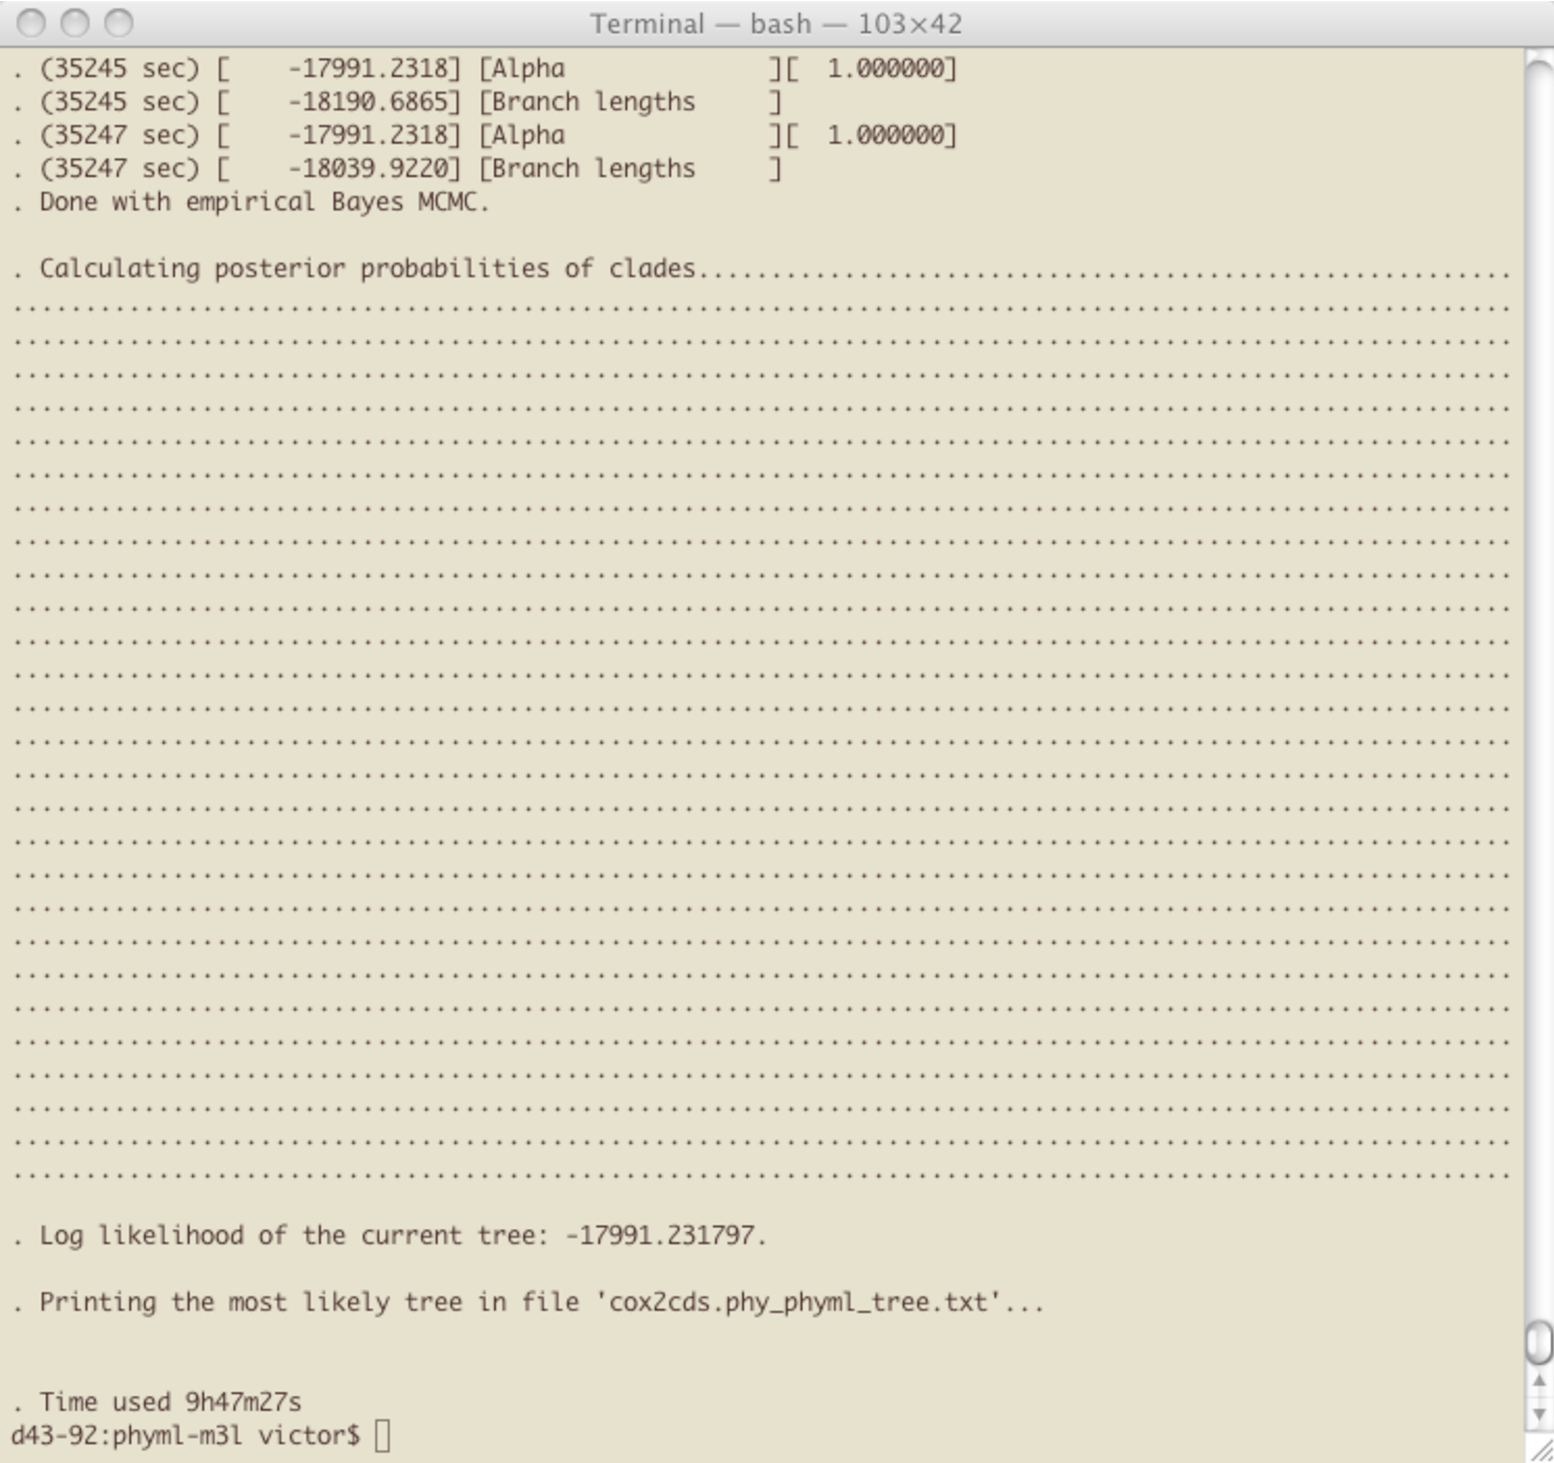
\includegraphics[width=5.5 in]{GRAPHICS/b7.pdf}
\caption{Eventually the analysis will finish and posterior probabilities of clades will be calculated.  The posterior probability of a clade equals the proportion of the MCMC samples in which that clade appears.}
\end{figure}
\clearpage


\begin{figure}[p]
\centering
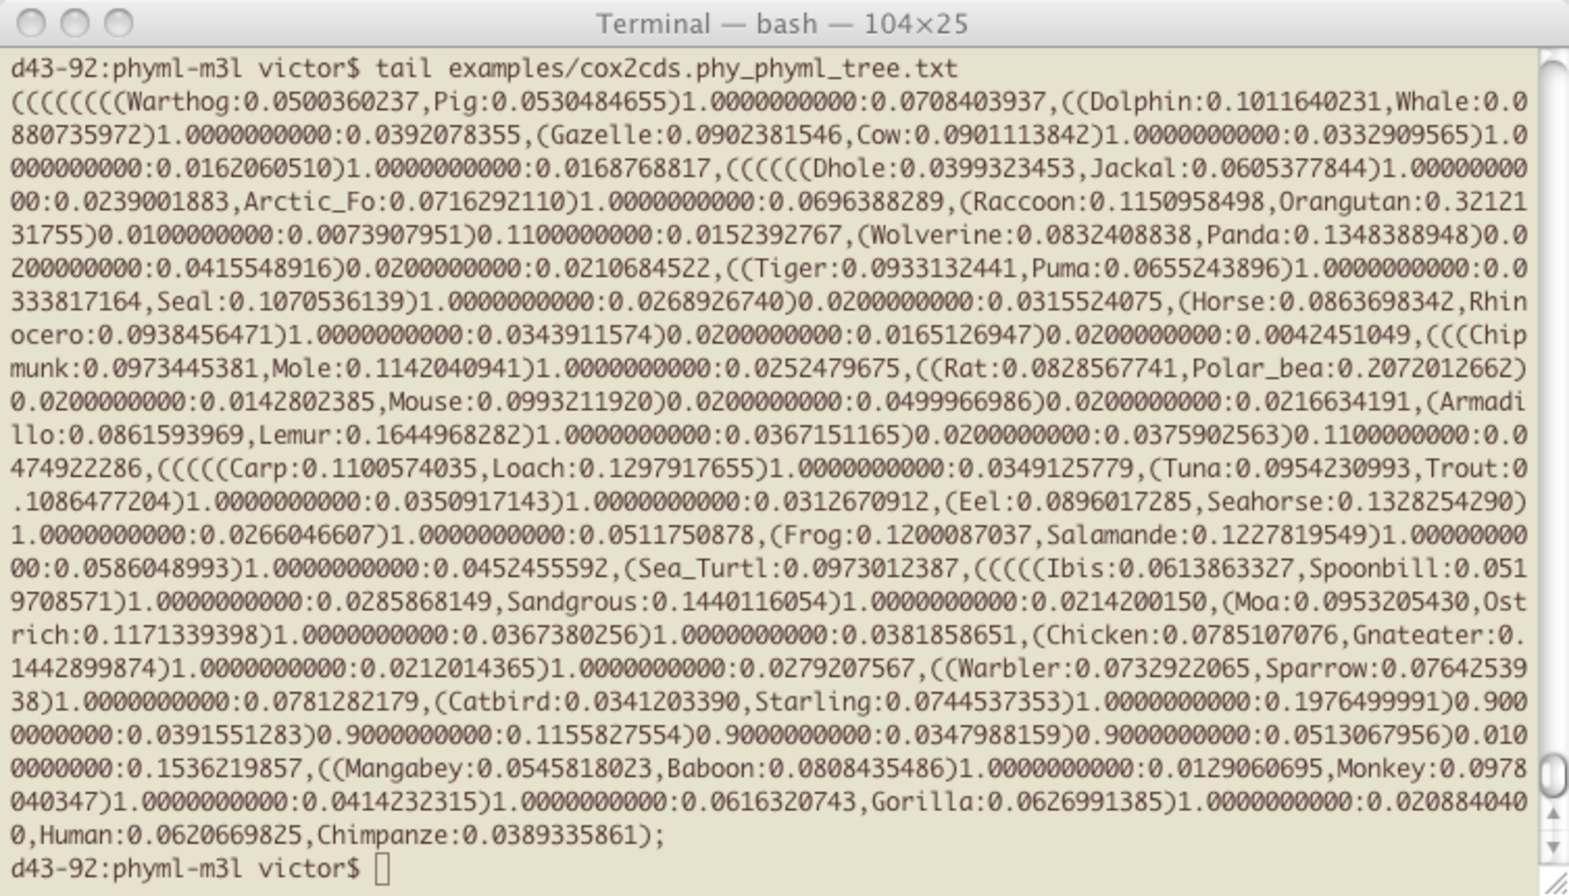
\includegraphics[width=5.5 in]{GRAPHICS/b8.pdf}
\caption{The clade posterior probabilities are printed with Newick-formatted phylogeny in the text file.  You can view that text file using your favorite text editor, or using unix commands such as \textit{tail}, \textit{less}, or \textit{cat}.}
\end{figure}
\clearpage

\subsection{Using simulated thermal annealing}
Simulated thermal annealing (STA) provides an alternative heuristic for optimizing the topology, branch lengths, and model parameters during phylogenetic inference.  For more information about STA in general, see \cite{Kirkpatrick1983} and \cite{kirkpatrick1984}.  For information about STA for optimizing phylogenies, see \cite{kolaczkowski2008}.

\medskip
\noindent Please be aware that STA is computationally demanding and can require several hours (or days!) to complete.

\medskip
The STA algorithm is configured using a large number of parameters, defining the length of computation and the shape of several probability distributions.  We have provided default values for all these parameters, but you can also specify custom values from the Terminal interface or the command-line.  Here we describe these parameters in detail:

\begin{description}

\item[Number of annealing stages]
\begin{verbatim}
( --num_anneal_stages )
\end{verbatim}

This integer value specifies how many intermediate temperatures will be evaluated as the temperature incrementally decreases from the starting temperature to the final temperature.  From some temperature $t_i$, the next temperature to be evaluated will equal:

$t_{i+1} = e^{ \frac{  log(\frac{t_f}{t_s})  }{  n   }   }$

where $t_f$ is the final temperature, $t_s$ is the starting temperature, and $n$ is the number of annealing stages.

\item[Starting temperature]
\begin{verbatim}
( --temp_start )
\end{verbatim}

The annealing algorithm will start the system with temperature equal to this value.

\item[Final temperature] 
\begin{verbatim}
( --temp_end )
\end{verbatim}

The annealing algorithm will terminate when the temperature eventually equals this value.

\item[Iterations per stage]
\begin{verbatim}
( --iters_per_stage )
\end{verbatim}

This value specifies how long the algorithm will dwell at each annealing stage.  In other words, at each temperature stage, the algorithm will propose (and potentially accept) a number of new parameter combinations equal to this value.

\item[Set-back interval size] 
\begin{verbatim}
( --set_back )
\end{verbatim}

The algorithm will ``set back'' the iteration counter for the current stage when the algorithm discovers a combination of parameters that yield a likelihood value higher than any previously observed likelihood.  By setting-back the counter, the algorithm will spend more time dwelling at this stage.  The rationale for this strategy is that we should not prematurely cool the system if the current temperature is still yielding optimal solutions.

\item[Acceptance ratio]
\begin{verbatim}
( --acc_ratio )
\end{verbatim}

This value specifies the acceptance ratio for new proposals of parameter values.  Larger values are more permissive to changes that result in worse likelihoods.  The probability of accepting a new proposal equals:

$P = e^{ \frac{L_{i+1} - L_{i}}{r - t} }$

where $L_{i+1}$ is the log likelihood of the proposed state, $L_i$ is the log likelihood of the current state, $r$ is the acceptance ratio, and $t$ is the current temperature of the system.

%\item[Starting tau value]
%\begin{verbatim}
%( --tau_start )
%\end{verbatim}

%asdfasdf

%\item[Ending tau value]
%\begin{verbatim}
%( --tau_end )
%\end{verbatim}

%asdfasdf

\item[Maximum alpha value]
\begin{verbatim}
( --max_alpha )
\end{verbatim}

This value specifies the maximum $\alpha$ value for a Dirichlet distribution.  The annealing algorithm draws random arrays of values from a Dirichlet distribution for the purposes of proposing a new set of state frequencies, a new set of relative substitution rates (for nucleotide data using HKY85 or GTR models), and a new set of branch lengths.

Do not confuse this $\alpha$ value with the $\alpha$ parameter in the gamma-distributed model of among-site rate variation.

\item[Branch length sigma value]
\begin{verbatim}
( --brlen_sigma )
\end{verbatim}

This value specifies the $\sigma$ value for describing a Gaussian distribution from which random branch lengths will be drawn to generate a new annealing proposal.

\item[P-invar sigma value]
\begin{verbatim}
( --pinvar_sigma )
\end{verbatim}

This value specifies the $\sigma$ value for describing a Gaussian distribution from which a random proportion of invariant sites will be drawn to generate a new annealing proposal.  This value is only valid if the invariant sites model is enabled.

\item[Gamma sigma value]
\begin{verbatim}
( --gamma_sigma )
\end{verbatim}

This value specifies the $\sigma$ value for describing a Gaussian distribution from which a random $\alpha$ value will be drawn to generate a gamma-distributed set of evolutionary rates.  This value is only valid if the gamma-distributed model is enabled.

%\item[Emig sigma value]
%\begin{verbatim}
%( --emig_sigma )
%\end{verbatim}

\item[Probability of stepping . .] .

At each iteration, the annealing algorithm generates a new proposed combination of parameter values, where each parameter value is probabilistically perturbed from the current set of parameter values.  The probability of perturbing, or ``stepping,'' each parameter is defined by a unique value; these values are described below.

\begin{verbatim}
--prob_topology
\end{verbatim}
Probability of proposing a new topology.

\begin{verbatim}
--prob_spr
\end{verbatim}
Probability of proposing a new tree using subtree pruning and regrafting (SPR).

\begin{verbatim}
--prob_brlen
\end{verbatim}
Probability of proposing a new set of branch lengths.

\begin{verbatim}
--prob_kappa
\end{verbatim}
Probability of proposing a new $\kappa$ value (for nucleotide data), where $\kappa$ is the ratio of transitions to transversions.

\begin{verbatim}
--prob_lambda
\end{verbatim}
Probability of proposing a new $\lambda$ value (for nucleotide data), where $\lambda$ defines the ratio of transitions to transversions in the F84 and TN93 models.

\begin{verbatim}
--prob_gamma
\end{verbatim}
Probability of proposing a new $\alpha$ value for describing the shape of the gamma-distribution for among site rate heterogeneity.  This value is only value if the gamma-distributed model is enabled.

\begin{verbatim}
--prob_rr
\end{verbatim}
Probability of proposing a new set of relative substitution rates (for nucleotide data).

\begin{verbatim}
--prob_rate_proportions
\end{verbatim}
Probability of proposing a new set of proportions for the gamma-distributed model of among site rate variation.

\begin{verbatim}
--prob_pinvar
\end{verbatim}
Probability of proposing a new proportion of invariant sites.  This value is only valid if the invariant-sites model is enabled.

\begin{verbatim}
--prob_pi
\end{verbatim}
Probability of proposing a new set of relative state frequencies.  This value is only valid if the state frequencies are not fixed.

\end{description}




\pagebreak
\section{Frequently Asked Questions}
\subsection{Why is this software named PhyML+M3L?}

The name ``M3L'' was originally M$^3$L (or M ``cubed'' L), standing for \textit{m}ixed \textit{m}odel \textit{m}aximum \textit{l}ikelihood.
%We started this project with the primary goal of implementing the multiple branch length model within PhyML.  Early on, we considered naming the project \textit{MBL}, for \textit{m}ultiple \textit{b}ranch \textit{l}engths.  Unfortunately, MBL is a poor keyword within the World Wide Web: (1) MBL are the initials of the Marine Biological Laboratory in Woods Hole, Maryland, (2) MBL is the name of a high-end audio components company in Germany, (3) MBL is a mispelling of the initials for Major League Baseball, and (4) \texttt{www.mbl.org} is a URL pointing to the Mouse Brain Library project.  We considered other project names, all of which are too ungainly to list here.  Eventually, we observed that the character `3' looks similar to the letter `B'.  Furthermore, the keyword \textit{M3L} is relatively unique within the World Wide Web.  M3L is the model name of a bicycle manufactured by Brompton Bicycles Ltd; M3L is also the name of a Maryland-based corporation providing ``mission support services.''  The name M3L is especially unique when paired with relevant keywords, such as \textit{phylogenetics}, \textit{likelihood}, or \textit{evolution}.  
M3L's project scope later grew to include the empirical Bayes MCMC sampler and multiprocessor parallelization.  At that point, we decided to keep the M3L moniker, despite the fact that M3L does not capture the entire project scope.

\subsection{How do I visualize a phylogeny with mixed branch lengths?}

Unfortunately, we do not know of any software for visualizing phylogenies with mixed branch lengths.  If your tree has only one branch length category, we recommend using the software FigTree:

\begin{verbatim}
         http://tree.bio.ed.ac.uk/software/figtree/
\end{verbatim}

\subsection{What about Windows?}

We have not tested PhyML or PhyML+M3L on Windows PCs.  In theory, you should be able to download the C source code and build the application yourself.  If you find success running our software on Windows, send us an email; we would love to know it works!

\subsection{I cannot compile the source code! I get an error relating to the `gsl', `libgsl', or the GNU Scientific Library.}

The +M3L extensions heavily employ methods from the GNU Scientific Library (GSL).  Among other features, the GSL provides useful C code for sampling random numbers from distributions.  On some -ix operating systems, including some distributions of Linux, the GSL BLAS library is installed in unique locations.  If your C compiler (such as \textbf{gcc} or \textbf{g++}) is complaining about missing references from GSL, try opening the file named `Makefile.am' and add the following tag to the `AM\_LDFLAGS' line:

\begin{verbatim}
         -lgslcblas
\end{verbatim}

\noindent In other words, transform this original line:

\begin{verbatim}
          AM_LDFLAGS=-lm -lgsl
\end{verbatim}

\noindent . . . into this new line:

\begin{verbatim}
          AM_LDFLAGS=-lm -lgsl -lgslcblas
\end{verbatim}

\pagebreak
\bibliography{/Users/victor/BIB_LIBRARY/MyBibTex/MyBibTex}
\bibliographystyle{apalike}

\end{document}